\section{บทที่ 5 การวิเคราะห์ผลตอบสนองชั่วครู่และข้อกำหนดสมรรถนะ}

% ให้สัญลักษณ์คณิตศาสตร์ Unicode ที่ใช้ในบทนี้แสดงด้วยฟอนต์คณิตศาสตร์
\catcode`τ=\active \protected\defτ{\ensuremath{\tau}}
\catcode`ζ=\active \protected\defζ{\ensuremath{\zeta}}
\catcode`ω=\active \protected\defω{\ensuremath{\omega}}
\catcode`Ω=\active \protected\defΩ{\ensuremath{\Omega}}
\catcode`μ=\active \protected\defμ{\ensuremath{\mu}}
\catcode`→=\active \protected\def→{\ensuremath{\to}}
\catcode`≤=\active \protected\def≤{\ensuremath{\le}}
\catcode`≥=\active \protected\def≥{\ensuremath{\ge}}
\catcode`≈=\active \protected\def≈{\ensuremath{\approx}}
\catcode`±=\active \protected\def±{\ensuremath{\pm}}

\noindent
\begin{tabular}{@{}ll@{}}
\textbf{ชื่อบทภาษาอังกฤษ:} & Transient Response Analysis and Performance Specifications \\
\textbf{รายวิชา:} & ระบบควบคุม (Control Systems)
\end{tabular}




\subsection{1. แนวคิดสำคัญของบท}

ในบทที่ 3 และบทที่ 4 นักศึกษาได้เรียนรู้วิธีสร้างแบบจำลองทางคณิตศาสตร์ของระบบควบคุมในรูปฟังก์ชันถ่ายโอน (Transfer Function) และวิธีลดรูปแผนภาพบล็อกหรือกราฟการไหลของสัญญาณให้เหลือฟังก์ชันถ่ายโอนเดียวที่แสดงความสัมพันธ์ระหว่างสัญญาณเข้าและสัญญาณออกของระบบ บทนี้จะนำฟังก์ชันถ่ายโอนที่ได้มาวิเคราะห์ \textbf{พฤติกรรมของระบบในโดเมนเวลา (Time-Domain Behavior)} โดยเฉพาะช่วงเวลาที่ระบบกำลังปรับตัวจากสภาวะเริ่มต้นไปสู่สภาวะคงตัว ซึ่งเรียกว่า \textbf{ผลตอบสนองชั่วครู่ (Transient Response)}

การเข้าใจผลตอบสนองชั่วครู่มีความสำคัญอย่างยิ่งต่อวิศวกรระบบควบคุม เพราะระบบวิศวกรรมจริง เช่น มอเตอร์ไฟฟ้า ระบบลิฟต์ ระบบควบคุมอุณหภูมิ หรือหุ่นยนต์ ล้วนต้องพิจารณาไม่เพียงว่าระบบจะไปถึงค่าที่ต้องการหรือไม่ (สภาวะคงตัว) แต่ยังต้องพิจารณาว่าระบบไปถึงค่านั้น \textbf{เร็วเพียงใด มีการแกว่งเกินค่าเป้าหมายหรือไม่ และสงบนิ่งเข้าสู่ค่าคงตัวภายในเวลาที่ยอมรับได้หรือไม่} คุณลักษณะเหล่านี้ถูกกำหนดเป็นตัวเลขเชิงปริมาณที่เรียกว่า \textbf{ข้อกำหนดสมรรถนะ (Performance Specifications)} ซึ่งวิศวกรใช้เป็นเกณฑ์ในการออกแบบและปรับแต่งระบบควบคุมให้ตอบสนองความต้องการของงานจริง

บทนี้ครอบคลุมการวิเคราะห์ระบบอันดับหนึ่งและอันดับสอง การจำแนกประเภทของการตอบสนอง การคำนวณข้อกำหนดสมรรถนะ และการวิเคราะห์ความผิดพลาดคงตัว ซึ่งเป็นพื้นฐานสำคัญก่อนเข้าสู่การออกแบบและปรับแต่งตัวควบคุมในบทถัดไป



\subsection{2. ความรู้พื้นฐานก่อนเรียน}

ก่อนเรียนบทนี้ นักศึกษาควรมีความรู้พื้นฐานดังต่อไปนี้

\begin{itemize}
    \item การแปลงลาปลาซ (Laplace Transform) และการแปลงผกผัน (Inverse Laplace Transform) เบื้องต้น รวมถึงการแยกเศษส่วนย่อย (Partial Fraction Expansion)
    \item แนวคิดฟังก์ชันถ่ายโอน (Transfer Function) จากบทที่ 3
    \item การลดรูปแผนภาพบล็อกและกราฟการไหลของสัญญาณจากบทที่ 4
    \item จำนวนเชิงซ้อน (Complex Numbers) และการอ่านตำแหน่งโพล-ซีโรบนระนาบ s (s-plane)
    \item สมการเชิงอนุพันธ์เชิงเส้นอันดับหนึ่งและอันดับสองเบื้องต้น
    \item ความรู้พื้นฐานวงจรไฟฟ้า ตัวต้านทาน ตัวเก็บประจุ และตัวเหนี่ยวนำ (R, L, C)
\end{itemize}



\subsection{3. คำสำคัญประจำบท}

\begin{table}[htbp]
    \centering
    \begin{tabularx}{\textwidth}{@{}>{\raggedright\arraybackslash}p{0.22\textwidth}>{\raggedright\arraybackslash}p{0.25\textwidth}>{\raggedright\arraybackslash}X@{}}
        \hline
        \textbf{คำศัพท์ภาษาไทย} & \textbf{English Term} & \textbf{ความหมายโดยย่อ} \\
        \hline
        ผลตอบสนองชั่วครู่ & Transient Response & ส่วนของผลตอบสนองที่เปลี่ยนแปลงตามเวลาก่อนเข้าสู่สภาวะคงตัว \\
        ผลตอบสนองคงตัว & Steady-State Response & ส่วนของผลตอบสนองเมื่อเวลาผ่านไปนานพอ \\
        ค่าคงเวลา & Time Constant (τ) & เวลาที่ระบบอันดับหนึ่งตอบสนองได้ 63.2\% ของค่าสุดท้าย \\
        อัตราส่วนหน่วง & Damping Ratio (ζ) & ค่าที่บ่งชี้ระดับการหน่วงของระบบอันดับสอง \\
        ความถี่ธรรมชาติไม่หน่วง & Natural Frequency (ωn) & ความถี่ที่ระบบจะแกว่งหากไม่มีการหน่วง \\
        ความถี่หน่วง & Damped Frequency (ωd) & ความถี่การแกว่งจริงที่สังเกตได้เมื่อมีการหน่วง \\
        ระบบหน่วงน้อยกว่าวิกฤต & Underdamped System & ระบบที่ 0 < ζ < 1 มีการแกว่งก่อนเข้าสู่ค่าคงตัว \\
        ระบบหน่วงวิกฤต & Critically Damped System & ระบบที่ ζ = 1 เข้าสู่ค่าคงตัวเร็วที่สุดโดยไม่แกว่ง \\
        ระบบหน่วงมากกว่าวิกฤต & Overdamped System & ระบบที่ ζ > 1 เข้าสู่ค่าคงตัวช้าโดยไม่แกว่ง \\
        เวลาขึ้น & Rise Time (tr) & เวลาที่ผลตอบสนองเพิ่มจากค่าต่ำไปสู่ค่าสูงใกล้ค่าสุดท้าย \\
        เวลาสูงสุด & Peak Time (tp) & เวลาที่ผลตอบสนองมีค่าสูงสุดครั้งแรก \\
        เปอร์เซ็นต์การพุ่งเกิน & Percent Overshoot (\%OS) & ร้อยละของค่าที่พุ่งเกินค่าสุดท้ายเทียบกับค่าสุดท้าย \\
        เวลาเข้าสู่ภาวะคงตัว & Settling Time (ts) & เวลาที่ผลตอบสนองเข้าสู่ช่วงยอมรับรอบค่าสุดท้ายอย่างถาวร \\
        ความผิดพลาดคงตัว & Steady-State Error (ess) & ผลต่างระหว่างสัญญาณอ้างอิงกับผลตอบสนองเมื่อเวลาผ่านไปนาน \\
        ระบบชนิดที่ & System Type & จำนวนตัวรวมสัญญาณ (โพลที่ s = 0) ในฟังก์ชันถ่ายโอนวงเปิด \\
        ค่าคงที่ความผิดพลาด & Error Constant (Kp, Kv, Ka) & ค่าคงที่ที่ใช้คำนวณความผิดพลาดคงตัวสำหรับสัญญาณอ้างอิงแต่ละแบบ \\
        \hline
    \end{tabularx}
\end{table}



\subsection{4. ผลลัพธ์การเรียนรู้ประจำบท}

เมื่อเรียนจบบทนี้ นักศึกษาสามารถ...

\begin{itemize}
    \item \textbf{CLO1:} อธิบายลักษณะและที่มาของผลตอบสนองชั่วครู่ของระบบอันดับหนึ่งและระบบอันดับสองได้อย่างถูกต้อง
    \item \textbf{CLO2:} คำนวณค่าคงเวลา (τ) อัตราส่วนหน่วง (ζ) และความถี่ธรรมชาติ (ωn) จากฟังก์ชันถ่ายโอนที่กำหนดให้
    \item \textbf{CLO3:} จำแนกประเภทของการตอบสนองของระบบอันดับสอง (Underdamped, Critically Damped, Overdamped) จากค่าพารามิเตอร์หรือตำแหน่งโพล
    \item \textbf{CLO4:} คำนวณข้อกำหนดสมรรถนะ ได้แก่ Rise Time, Peak Time, Percent Overshoot และ Settling Time จากพารามิเตอร์ของระบบ และประยุกต์ใช้ในการออกแบบเบื้องต้น
    \item \textbf{CLO5:} วิเคราะห์ความผิดพลาดคงตัวของระบบวงปิด จำแนกชนิดของระบบ (System Type) และคำนวณค่าคงที่ความผิดพลาด
    \item \textbf{CLO6:} ทดลองวัดผลตอบสนองชั่วครู่จริงจากวงจร RC และ RLC ด้วยออสซิลโลสโคป และเปรียบเทียบผลกับค่าที่คำนวณได้จากทฤษฎีและจากการจำลองด้วย MATLAB
\end{itemize}

\subsubsection{ตารางเชื่อมโยงผลลัพธ์การเรียนรู้กับเนื้อหาและการประเมิน}

\begin{table}[htbp]
    \centering
    \small
    \begin{tabularx}{\textwidth}{@{}>{\raggedright\arraybackslash}p{0.10\textwidth}*{4}{>{\raggedright\arraybackslash}X}@{}}
        \hline
        \textbf{ผลลัพธ์การเรียนรู้ประจำบท} & \textbf{เนื้อหาที่เกี่ยวข้อง} & \textbf{กิจกรรมการเรียนรู้} & \textbf{วิธีประเมิน} & \textbf{หลักฐานการเรียนรู้} \\
        \hline
        CLO1 & หัวข้อ 7.1, 7.2 ระบบอันดับหนึ่งและอันดับสอง & บรรยาย, อภิปรายกราฟผลตอบสนอง & คำถามทบทวนข้อ 1–3 & คำตอบปากเปล่า/ลายลักษณ์อักษรในชั้นเรียน \\
        CLO2 & หัวข้อ 7.1–7.3 สมการมาตรฐานและการเทียบสัมประสิทธิ์ & ตัวอย่างที่ 1–2, แบบฝึกหัดพื้นฐาน & แบบฝึกหัดระดับพื้นฐาน & ใบงานคำนวณ \\
        CLO3 & หัวข้อ 7.3 ประเภทของการตอบสนอง & วิเคราะห์ตำแหน่งโพลบนระนาบ s & แบบฝึกหัดระดับพื้นฐานและวิเคราะห์ & ใบงาน/Exit ticket \\
        CLO4 & หัวข้อ 7.4 ข้อกำหนดสมรรถนะ & ตัวอย่างที่ 3–4, กิจกรรมปฏิบัติการที่ 2 & แบบฝึกหัดระดับวิเคราะห์และประยุกต์ & ใบงาน, รายงานผลปฏิบัติการ \\
        CLO5 & หัวข้อ 7.5 ความผิดพลาดคงตัว & ตัวอย่างที่ 5, แบบฝึกหัดระดับวิเคราะห์ & แบบฝึกหัดระดับวิเคราะห์และประยุกต์ & ใบงานคำนวณ \\
        CLO6 & หัวข้อ 7.6 การจำลองด้วย MATLAB, กิจกรรมปฏิบัติการที่ 1–2 & ปฏิบัติการวัดค่าจริงและจำลองด้วยซอฟต์แวร์ & เกณฑ์การประเมินปฏิบัติการ & รายงานผลปฏิบัติการ, กราฟเปรียบเทียบ \\
        \hline
    \end{tabularx}
\end{table}



\subsection{5. แผนผังเนื้อหาของบท}

ลำดับเนื้อหาของบทนี้จัดเรียงจากพื้นฐานไปสู่การวิเคราะห์และประยุกต์ใช้ ดังนี้

\begin{enumerate}
    \item ระบบอันดับหนึ่ง (First-Order System) → ค่าคงเวลา τ → Step Response
    \item ระบบอันดับสอง (Second-Order System) → รูปแบบมาตรฐาน → ζ และ ωn
    \item ประเภทของการตอบสนอง (Underdamped / Critically Damped / Overdamped)
    \item ข้อกำหนดสมรรถนะ (tr, tp, \%OS, ts) และความสัมพันธ์กับ ζ, ωn
    \item การจำลองผลตอบสนองด้วย MATLAB
    \item ความผิดพลาดคงตัว (ess) → System Type → ค่าคงที่ความผิดพลาด (Kp, Kv, Ka)
    \item การประยุกต์ใช้ในงานจริงและกิจกรรมปฏิบัติการวัดผลตอบสนองจากวงจร RC/RLC จริง
\end{enumerate}

\newpage

\subsection{6. บทนำ}

ระบบควบคุมทุกระบบเมื่อได้รับสัญญาณเข้าที่เปลี่ยนแปลง เช่น สัญญาณขั้นบันได (Step Input) จะแสดงผลตอบสนองที่ประกอบด้วยสองส่วนเสมอ คือ ส่วนที่เปลี่ยนแปลงตามเวลาในช่วงแรก (ผลตอบสนองชั่วครู่) และส่วนที่คงที่เมื่อเวลาผ่านไปนานพอ (ผลตอบสนองคงตัว) ลองพิจารณาลิฟต์โดยสารที่ถูกสั่งให้เคลื่อนที่ไปยังชั้นเป้าหมาย ลิฟต์ไม่ได้กระโดดไปถึงชั้นเป้าหมายทันที แต่จะเร่งความเร็ว แล่นด้วยความเร็วคงที่ ชะลอความเร็ว และอาจหยุดเลยตำแหน่งเป้าหมายเล็กน้อยก่อนขยับกลับมาหยุดสนิท พฤติกรรมทั้งหมดนี้คือผลตอบสนองชั่วครู่ ซึ่งเป็นสิ่งที่วิศวกรต้องออกแบบให้เหมาะสม เพราะหากลิฟต์เร่งเร็วเกินไปผู้โดยสารจะรู้สึกไม่สบาย หากหยุดเลยตำแหน่งมากเกินไปจะเกิดอันตราย และหากใช้เวลานานเกินไปกว่าจะหยุดนิ่งจะทำให้ประสิทธิภาพการใช้งานลดลง

ในทางคณิตศาสตร์ ผลตอบสนองชั่วครู่ของระบบผูกติดกับตำแหน่งโพลของฟังก์ชันถ่ายโอนบนระนาบ s โดยตรง ระบบอันดับหนึ่งมีโพลเดียวบนแกนจริง ทำให้ผลตอบสนองเป็นเลขชี้กำลังอย่างง่าย ในขณะที่ระบบอันดับสองมีโพลคู่ที่อาจเป็นจำนวนจริงหรือจำนวนเชิงซ้อนคู่สังยุค ทำให้เกิดพฤติกรรมได้หลายรูปแบบตั้งแต่การเข้าสู่ค่าคงตัวอย่างราบเรียบไปจนถึงการแกว่งก่อนสงบนิ่ง บทนี้จะแสดงให้เห็นว่าพารามิเตอร์เพียงสองตัว คือ อัตราส่วนหน่วง (ζ) และความถี่ธรรมชาติ (ωn) สามารถอธิบายพฤติกรรมของระบบอันดับสองได้อย่างครบถ้วน และนำไปสู่การคำนวณข้อกำหนดสมรรถนะที่ใช้ในงานออกแบบจริง



\subsection{7. เนื้อหาหลัก}

\subsubsection{7.1 ผลตอบสนองของระบบอันดับหนึ่ง (First-Order System Response)}

\textbf{นิยามและรูปแบบมาตรฐาน}

ระบบอันดับหนึ่งคือระบบที่ฟังก์ชันถ่ายโอนมีตัวส่วนเป็นพหุนามดีกรีหนึ่งใน s เขียนในรูปมาตรฐานได้เป็น

\[
G(s) = \frac{K}{\tau s + 1}
\]

โดยที่ $K$ คืออัตราขยายสถานะคงตัว (Steady-State Gain) และ $\tau$ คือ \textbf{ค่าคงเวลา (Time Constant)} มีหน่วยเป็นวินาที (s) ค่าคงเวลาเป็นพารามิเตอร์เดียวที่กำหนดความเร็วในการตอบสนองของระบบอันดับหนึ่งทั้งหมด

\textbf{การหาผลตอบสนองต่อสัญญาณขั้นบันได}

เมื่อป้อนสัญญาณขั้นบันไดหนึ่งหน่วย $R(s) = 1/s$ เข้าสู่ระบบที่มี $K=1$ จะได้

\[
C(s) = \frac{1}{s(\tau s+1)}
\]

แยกเศษส่วนย่อย

\[
C(s) = \frac{1}{s} - \frac{\tau}{\tau s+1} = \frac{1}{s} - \frac{1}{s+\frac{1}{\tau}}
\]

แปลงผกผันลาปลาซจะได้ผลตอบสนองในโดเมนเวลา

\[
c(t) = 1 - e^{-t/\tau}, \qquad t \ge 0
\]

\textbf{ความหมายทางกายภาพของ τ}

เมื่อแทน $t=\tau$ จะได้ $c(\tau) = 1-e^{-1} = 0.632$ นั่นคือ \textbf{ค่าคงเวลาคือเวลาที่ผลตอบสนองไปถึง 63.2\% ของค่าสุดท้าย} และเมื่อเวลาผ่านไปหลายเท่าของ τ ผลตอบสนองจะเข้าใกล้ค่าสุดท้ายมากขึ้นตามตาราง

\begin{table}[htbp]
    \centering
    \begin{tabular}{lr}
        \hline
        \textbf{เวลา} & \textbf{เปอร์เซ็นต์ของค่าสุดท้าย} \\
        \hline
        $t = \tau$ & 63.2\% \\
        $t = 2\tau$ & 86.5\% \\
        $t = 3\tau$ & 95.0\% \\
        $t = 4\tau$ & 98.2\% \\
        $t = 5\tau$ & 99.3\% \\
        \hline
    \end{tabular}
\end{table}

ในทางปฏิบัติวิศวกรมักถือว่าระบบอันดับหนึ่ง \textbf{เข้าสู่สภาวะคงตัว} เมื่อเวลาผ่านไปประมาณ $4\tau$ ถึง $5\tau$ ขึ้นกับเกณฑ์ความคลาดเคลื่อนที่ยอมรับ (2\% หรือ 1\% ตามลำดับ)

% [รูปที่ 1: กราฟผลตอบสนองต่อสัญญาณขั้นบันไดของระบบอันดับหนึ่ง]
% ประเภทภาพ: Graph
% ตำแหน่งที่แนะนำ: หลังสมการ $c(t)=1-e^{-t/\tau}$ ในหัวข้อ 7.1
% วัตถุประสงค์การเรียนรู้: ให้ผู้เรียนเห็นความสัมพันธ์ระหว่างค่าคงเวลา τ กับรูปร่างของกราฟผลตอบสนอง และจดจำจุด 63.2% ได้
% คำอธิบายภาพ: กราฟแกนนอนเป็นเวลา t (มีเส้นบอกตำแหน่ง τ, 2τ, 3τ, 4τ, 5τ) แกนตั้งเป็น c(t) ตั้งแต่ 0 ถึง 1 เส้นกราฟเริ่มจาก 0 โค้งขึ้นแบบเลขชี้กำลังเข้าใกล้ 1 มีเส้นประแนวนอนที่ 0.632 ตัดกับเส้นกราฟที่ตำแหน่ง t=τ
% องค์ประกอบที่ต้องมี: แกน t, แกน c(t), เส้นโค้งผลตอบสนอง, เส้นประระบุ 63.2% และตำแหน่ง τ, เส้นประเส้นกำกับ (Asymptote) ที่ c(t)=1
% ข้อความหรือป้ายกำกับ: "63.2%", "τ", "2τ", "3τ", "4τ", "5τ", "c(t) = 1 − e^(−t/τ)"
% ภาษาของป้ายกำกับ: ไทยและอังกฤษ
% สัดส่วนภาพ: 4:3
% Image Generation Prompt: Clean educational engineering graph, exponential rise curve from 0 to 1 approaching an asymptote, dashed horizontal line at 0.632 intersecting the curve at time constant tau, x-axis labeled with tau, 2tau, 3tau, 4tau, 5tau, minimalist technical illustration style, white background, labeled axes
% Graph Generation Prompt: พล็อตฟังก์ชัน $c(t)=1-e^{-t/\tau}$ โดยกำหนด τ=1 (normalized), ช่วงเวลา $t \in [0, 5\tau]$, แกนตั้ง $c(t) \in [0,1]$, ทำเครื่องหมายจุดที่ t=τ,2τ,3τ,4τ,5τ
% Alt Text: กราฟแสดงผลตอบสนองต่อสัญญาณขั้นบันไดของระบบอันดับหนึ่ง เพิ่มขึ้นแบบเลขชี้กำลังจาก 0 ถึง 1 โดยถึง 63.2% ที่เวลาเท่ากับหนึ่งค่าคงเวลา

\begin{figure}[htbp]
    \centering
    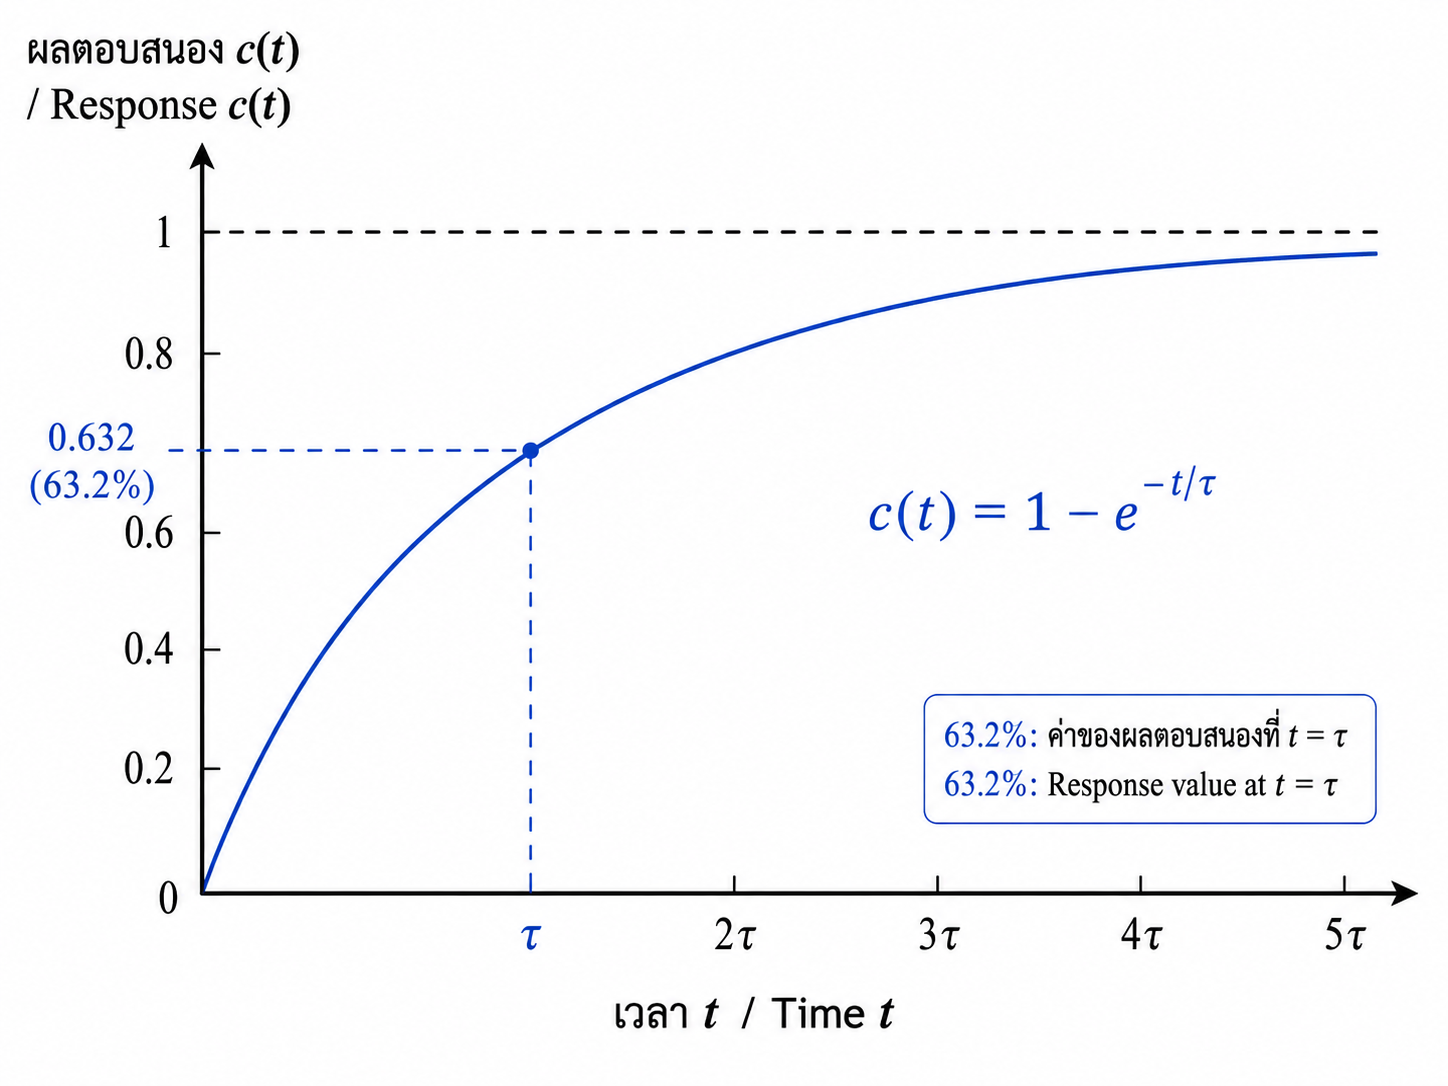
\includegraphics[width=0.8\textwidth]{images/chapter5/figure-01.png}
    \caption{กราฟผลตอบสนองต่อสัญญาณขั้นบันไดของระบบอันดับหนึ่ง}
\end{figure}



\textbf{ตัวอย่างที่ 1 (พื้นฐาน): การหาค่าคงเวลาและเวลาที่ผลตอบสนองเข้าใกล้ค่าสุดท้าย}

โจทย์: ระบบวงปิดมีฟังก์ชันถ่ายโอน $T(s) = \dfrac{4}{s+4}$ จงหาค่าคงเวลา τ และเวลาที่ผลตอบสนองต่อสัญญาณขั้นบันไดหนึ่งหน่วยมีค่าถึง 90\% และ 95\% ของค่าสุดท้าย รวมถึง Settling Time ที่เกณฑ์ 2\%

\textit{ขั้นตอนที่ 1 วิเคราะห์ระบบ:} ระบบเป็นอันดับหนึ่ง มีโพลเดียวที่ $s=-4$

\textit{ขั้นตอนที่ 2 กำหนดตัวแปร:} ให้ $c(t)$ เป็นผลตอบสนองต่อสัญญาณขั้นบันไดหนึ่งหน่วย

\textit{ขั้นตอนที่ 3 เลือกหลักการ:} จัดรูป $T(s)$ ให้อยู่ในรูปมาตรฐาน $K/(\tau s+1)$

\textit{ขั้นตอนที่ 4 สร้างสมการ:} หารเศษและส่วนด้วย 4

\[
T(s) = \frac{4}{s+4} = \frac{1}{0.25s+1}
\]

\textit{ขั้นตอนที่ 5 จัดรูปสมการ:} เทียบกับรูปมาตรฐานได้ $\tau = 0.25$ วินาที และ $K=1$

\textit{ขั้นตอนที่ 6 แทนค่า/แปลงโดเมน:} ใช้ $c(t) = 1-e^{-t/\tau}$ ตั้งสมการหาค่า $t$ ที่ $c(t)=0.90$ และ $c(t)=0.95$

\[
1-e^{-t/\tau} = 0.90 \;\Rightarrow\; e^{-t/\tau} = 0.10 \;\Rightarrow\; t = \tau \ln(10)
\]

\[
1-e^{-t/\tau} = 0.95 \;\Rightarrow\; e^{-t/\tau} = 0.05 \;\Rightarrow\; t = \tau \ln(20)
\]

\textit{ขั้นตอนที่ 7 คำนวณ:}

\[
t_{90\%} = 0.25 \times 2.3026 = 0.576 \text{ s}, \qquad t_{95\%} = 0.25 \times 2.9957 = 0.749 \text{ s}
\]

Settling Time ที่เกณฑ์ 2\% ประมาณจาก $t_s \approx 4\tau = 4 \times 0.25 = 1.0$ วินาที

\textit{ขั้นตอนที่ 8 ตรวจสอบหน่วยและความสมเหตุสมผล:} หน่วยเป็นวินาทีสอดคล้องกับนิยามของเวลา และค่า $t_{90\%} < t_{95\%} < t_s$ ซึ่งเป็นไปตามลำดับที่ควรจะเป็น

\textit{ขั้นตอนที่ 9 แปลความหมาย:} ระบบนี้มีค่าคงเวลาเพียง 0.25 วินาที จึงเป็นระบบที่ตอบสนองเร็ว โดยจะเข้าใกล้ค่าสุดท้ายเกือบสมบูรณ์ภายในเวลาประมาณ 1 วินาที



\subsubsection{7.2 ผลตอบสนองของระบบอันดับสอง (Second-Order System Response)}

ระบบทางวิศวกรรมจำนวนมาก เช่น ระบบมอเตอร์ไฟฟ้าที่มีความเฉื่อยและความหน่วง หรือวงจร RLC มีฟังก์ชันถ่ายโอนแบบอันดับสอง ซึ่งเขียนในรูปมาตรฐาน (Standard Second-Order Form) ได้เป็น

\[
G(s) = \frac{\omega_n^2}{s^2 + 2\zeta\omega_n s + \omega_n^2}
\]

โดยที่

\begin{itemize}
    \item $\omega_n$ คือ \textbf{ความถี่ธรรมชาติไม่หน่วง (Undamped Natural Frequency)} มีหน่วยเป็น rad/s คือความถี่ที่ระบบจะแกว่งหากไม่มีความหน่วงใด ๆ
    \item $\zeta$ (ซีตา) คือ \textbf{อัตราส่วนหน่วง (Damping Ratio)} เป็นค่าไม่มีหน่วย บ่งชี้ระดับการหน่วงของระบบเทียบกับการหน่วงวิกฤต
\end{itemize}

สมการเอกลักษณ์ (Characteristic Equation) ของระบบคือ

\[
s^2 + 2\zeta\omega_n s + \omega_n^2 = 0
\]

แก้สมการหาโพลได้

\[
s_{1,2} = -\zeta\omega_n \pm \omega_n\sqrt{\zeta^2-1}
\]

\textbf{สมมติฐานและเงื่อนไขการใช้งาน:} สูตรและข้อกำหนดสมรรถนะในบทนี้อ้างอิงจากระบบอันดับสองมาตรฐานที่ไม่มีซีโรจำกัด (Finite Zero) และไม่มีโพลเพิ่มเติมอื่นนอกเหนือจากคู่โพลหลัก หากระบบจริงมีซีโรหรือโพลเพิ่มเติมที่อยู่ใกล้คู่โพลหลัก ค่าที่คำนวณได้จากสูตรเหล่านี้จะเป็นเพียงค่าประมาณ


\subsubsection{7.3 ประเภทของการตอบสนอง (Response Types)}

ค่าอัตราส่วนหน่วง $\zeta$ เป็นตัวกำหนดตำแหน่งของโพลบนระนาบ s และรูปแบบของผลตอบสนอง แบ่งออกเป็น 4 กรณี

\textbf{กรณีที่ 1: ไม่มีการหน่วง (Undamped, $\zeta = 0$)}
โพลเป็นจำนวนจินตภาพล้วน $s_{1,2}=\pm j\omega_n$ ระบบแกว่งตลอดไปโดยไม่ลดขนาดลง ไม่พบในระบบจริงที่มีการสูญเสียพลังงาน แต่ใช้เป็นกรณีอ้างอิงทางทฤษฎี

\textbf{กรณีที่ 2: หน่วงน้อยกว่าวิกฤต (Underdamped, $0 < \zeta < 1$)}
โพลเป็นจำนวนเชิงซ้อนคู่สังยุค

\[
s_{1,2} = -\zeta\omega_n \pm j\omega_n\sqrt{1-\zeta^2} = -\zeta\omega_n \pm j\omega_d
\]

โดยนิยาม \textbf{ความถี่หน่วง (Damped Frequency)}

\[
\omega_d = \omega_n\sqrt{1-\zeta^2}
\]

ผลตอบสนองต่อสัญญาณขั้นบันไดหนึ่งหน่วยมีรูปแบบ

\[
c(t) = 1 - \frac{e^{-\zeta\omega_n t}}{\sqrt{1-\zeta^2}}\sin(\omega_d t + \theta), \qquad \theta = \cos^{-1}\zeta
\]

ผลตอบสนองแบบนี้มีลักษณะแกว่งพุ่งเกินค่าสุดท้ายก่อนสงบนิ่งเข้าสู่ค่าคงตัว เป็นกรณีที่พบบ่อยที่สุดในระบบควบคุมจริงและเป็นกรณีหลักที่ใช้นิยามข้อกำหนดสมรรถนะในหัวข้อ 7.4

\textbf{กรณีที่ 3: หน่วงวิกฤต (Critically Damped, $\zeta = 1$)}
โพลซ้ำเป็นจำนวนจริง $s_{1,2}=-\omega_n$ ผลตอบสนองไม่มีการแกว่งและเข้าสู่ค่าคงตัวได้เร็วที่สุดในบรรดาระบบที่ไม่มีการพุ่งเกิน

\textbf{กรณีที่ 4: หน่วงมากกว่าวิกฤต (Overdamped, $\zeta > 1$)}
โพลเป็นจำนวนจริงสองค่าที่แตกต่างกัน

\[
s_{1,2} = -\zeta\omega_n \pm \omega_n\sqrt{\zeta^2-1}
\]

ผลตอบสนองเป็นผลรวมของเลขชี้กำลังสองพจน์ ไม่มีการแกว่ง แต่เข้าสู่ค่าคงตัวช้ากว่ากรณีหน่วงวิกฤต

% [รูปที่ 2: ตำแหน่งโพลบนระนาบ s สำหรับกรณีการหน่วงต่าง ๆ]
% ประเภทภาพ: Technical Illustration
% ตำแหน่งที่แนะนำ: หลังการอธิบายทั้งสี่กรณีในหัวข้อ 7.3
% วัตถุประสงค์การเรียนรู้: ให้ผู้เรียนเชื่อมโยงค่า ζ กับตำแหน่งโพลบนระนาบ s ได้โดยตรง
% คำอธิบายภาพ: ระนาบ s แสดงแกนจริง (Re) แนวนอนและแกนจินตภาพ (Im) แนวตั้ง แสดงตำแหน่งโพล 4 ชุด ได้แก่ โพลบนแกนจินตภาพ (ζ=0), โพลเชิงซ้อนคู่สังยุคในครึ่งซ้าย (0<ζ<1) พร้อมมุม θ จากแกนจินตภาพลบ, โพลซ้ำบนแกนจริงลบ (ζ=1), และโพลจริงสองตำแหน่งบนแกนจริงลบที่ระยะห่างต่างกัน (ζ>1)
% องค์ประกอบที่ต้องมี: แกน Re, แกน Im, จุดกากบาทแทนตำแหน่งโพลแต่ละกรณี, เส้นประรัศมี ωn จากจุดกำเนิดถึงโพลเชิงซ้อน, มุม θ = cos⁻¹ζ
% ข้อความหรือป้ายกำกับ: "ζ=0", "0<ζ<1", "ζ=1", "ζ>1", "ωn", "θ", "Re", "Im"
% ภาษาของป้ายกำกับ: ไทยและอังกฤษ
% สัดส่วนภาพ: 4:3
% Image Generation Prompt: Technical diagram of the complex s-plane showing pole locations for four damping cases: purely imaginary poles, complex conjugate pole pair in the left half plane with angle theta from the negative imaginary axis, repeated real pole, and two distinct real poles further left, engineering textbook style, labeled axes, minimalist line art
% Alt Text: แผนภาพระนาบ s แสดงตำแหน่งโพลสำหรับกรณี Undamped, Underdamped, Critically Damped และ Overdamped

\begin{figure}[htbp]
    \centering
    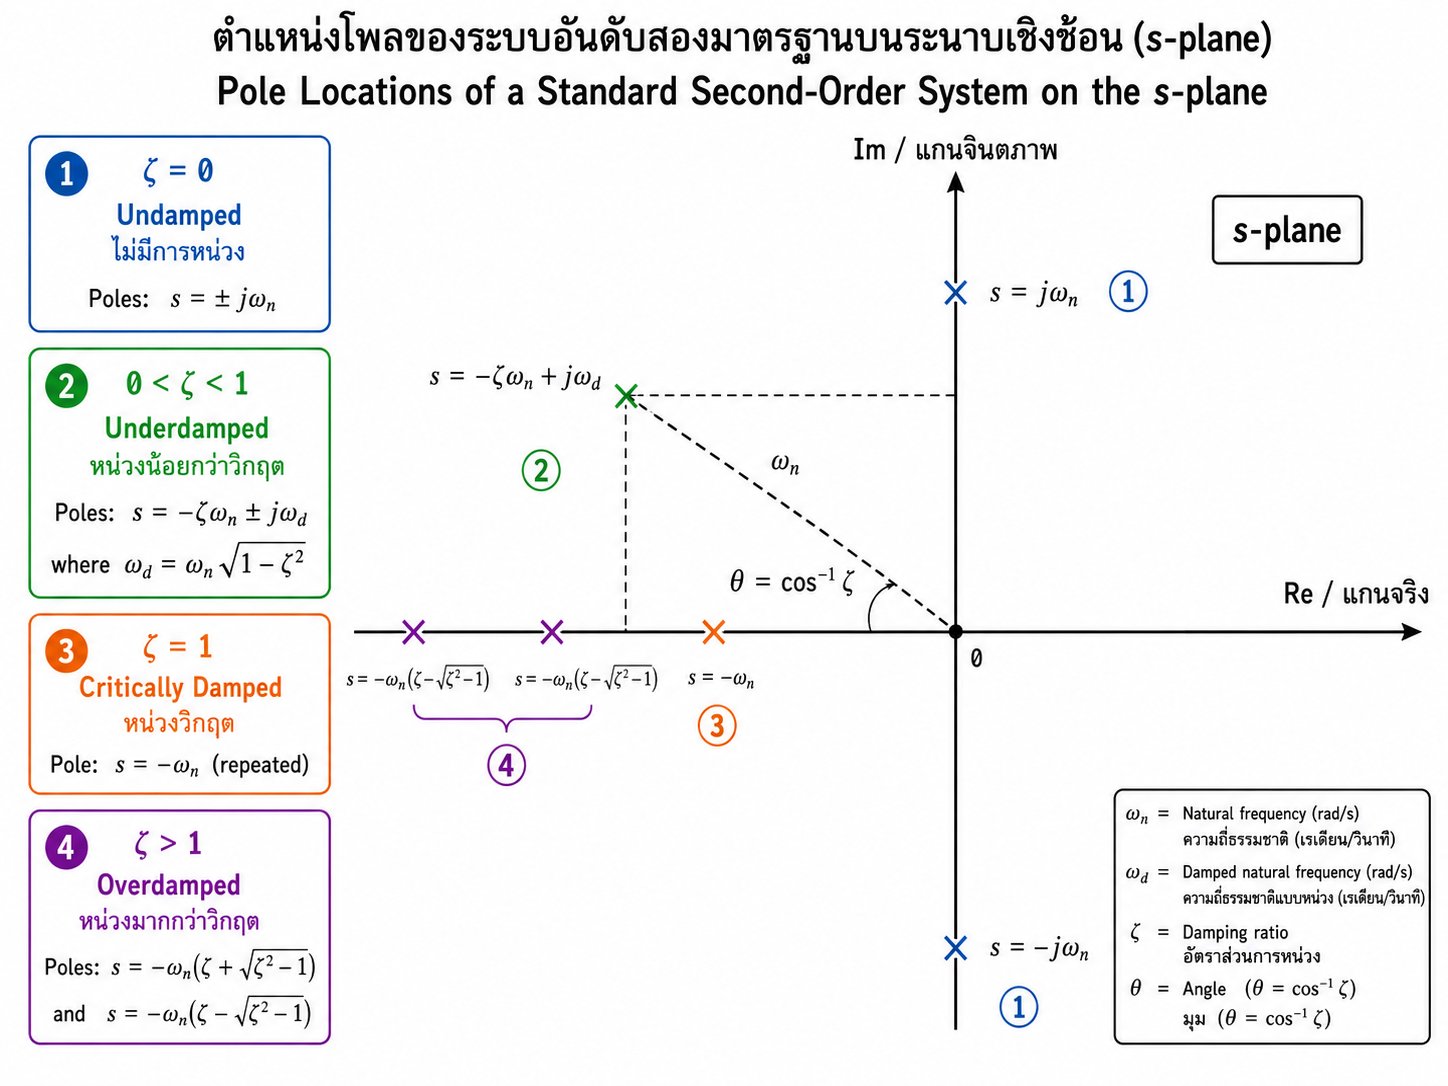
\includegraphics[width=0.8\textwidth]{images/chapter5/figure-02.png}
    \caption{ตำแหน่งโพลบนระนาบ s สำหรับกรณีการหน่วงต่าง ๆ}
\end{figure}

% [รูปที่ 3: กราฟเปรียบเทียบผลตอบสนองต่อสัญญาณขั้นบันไดสำหรับค่า ζ ต่าง ๆ]
% ประเภทภาพ: Graph
% ตำแหน่งที่แนะนำ: ต่อจากรูปที่ 2 ในหัวข้อ 7.3
% วัตถุประสงค์การเรียนรู้: ให้ผู้เรียนเห็นภาพรวมว่าเมื่อ ζ เปลี่ยนแปลง รูปร่างของกราฟผลตอบสนองเปลี่ยนไปอย่างไร
% คำอธิบายภาพ: กราฟแกนนอนเป็นเวลา $\omega_n t$ (Normalized Time) แกนตั้งเป็น c(t) มีเส้นกราฟหลายเส้นซ้อนกันสำหรับ ζ = 0 (แกว่งไม่ลดทอน), ζ = 0.2, ζ = 0.5, ζ = 0.7 (Underdamped ระดับต่าง ๆ), ζ = 1 (Critically Damped), ζ = 2 (Overdamped)
% องค์ประกอบที่ต้องมี: แกน ωn t, แกน c(t), เส้นกำกับ c(t)=1, เส้นกราฟหลายสีพร้อม Legend ระบุค่า ζ ของแต่ละเส้น
% ข้อความหรือป้ายกำกับ: "ζ=0", "ζ=0.2", "ζ=0.5", "ζ=0.7", "ζ=1", "ζ=2", "ωn t", "c(t)"
% ภาษาของป้ายกำกับ: ไทยและอังกฤษ
% สัดส่วนภาพ: 16:9
% Image Generation Prompt: Family of step response curves for a standard second order system at damping ratios 0, 0.2, 0.5, 0.7, 1, and 2, overlaid on one graph with normalized time axis, color-coded legend, engineering textbook style, clean white background
% Graph Generation Prompt: พล็อตสมการ $c(t)=1-\dfrac{e^{-\zeta\omega_n t}}{\sqrt{1-\zeta^2}}\sin(\omega_d t+\theta)$ สำหรับ ζ=0.2,0.5,0.7 และสมการกรณี ζ=1, ζ=2 ตามลำดับ ช่วงเวลา $\omega_n t \in [0,15]$ แกนตั้ง c(t) ตั้งแต่ 0 ถึงประมาณ 1.6
% Alt Text: กราฟเปรียบเทียบผลตอบสนองต่อสัญญาณขั้นบันไดของระบบอันดับสองที่ค่าอัตราส่วนหน่วงต่างกันหกค่า

\begin{figure}[htbp]
    \centering
    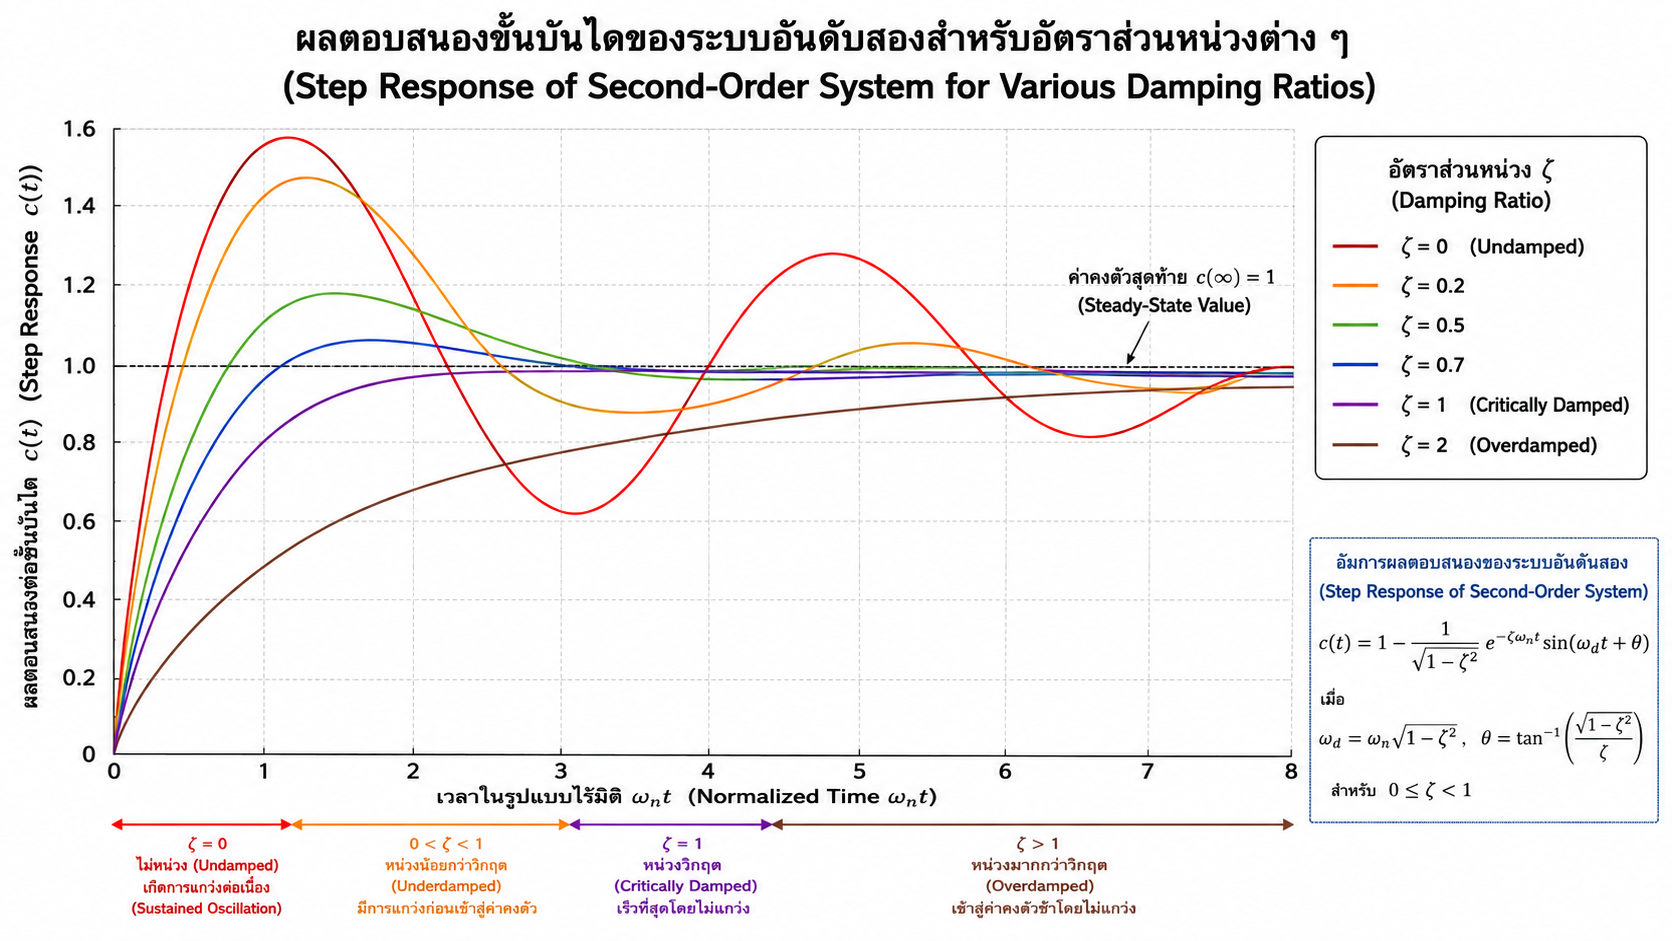
\includegraphics[width=0.8\textwidth]{images/chapter5/figure-03.png}
    \caption{กราฟเปรียบเทียบผลตอบสนองต่อสัญญาณขั้นบันไดสำหรับค่า ζ ต่าง ๆ}
\end{figure}



\textbf{ตัวอย่างที่ 2 (เชิงวิเคราะห์): การจำแนกประเภทการตอบสนองจากฟังก์ชันถ่ายโอน}

โจทย์: ระบบวงปิดมีฟังก์ชันถ่ายโอน $T(s) = \dfrac{36}{s^2+4.2s+36}$ จงหาค่า ζ, ωn, ωd และตำแหน่งโพล พร้อมระบุประเภทของการตอบสนอง

\textit{ขั้นตอนที่ 1 วิเคราะห์ระบบ:} เป็นระบบอันดับสองในรูปมาตรฐานอยู่แล้ว

\textit{ขั้นตอนที่ 2 กำหนดตัวแปร:} เทียบสัมประสิทธิ์กับ $\omega_n^2/(s^2+2\zeta\omega_n s+\omega_n^2)$

\textit{ขั้นตอนที่ 3 เลือกหลักการ:} การเทียบสัมประสิทธิ์พหุนามตัวส่วน

\textit{ขั้นตอนที่ 4 สร้างสมการ:} $\omega_n^2 = 36$ และ $2\zeta\omega_n = 4.2$

\textit{ขั้นตอนที่ 5 จัดรูปสมการ:} $\omega_n = \sqrt{36} = 6$ rad/s และ $\zeta = 4.2/(2\times 6)$

\textit{ขั้นตอนที่ 6 แทนค่า:} $\zeta = 4.2/12 = 0.35$

\textit{ขั้นตอนที่ 7 คำนวณ:}

\[
\omega_d = \omega_n\sqrt{1-\zeta^2} = 6\sqrt{1-0.1225} = 6\times 0.9367 = 5.62 \text{ rad/s}
\]

\[
s_{1,2} = -\zeta\omega_n \pm j\omega_d = -2.1 \pm j5.62
\]

\textit{ขั้นตอนที่ 8 ตรวจสอบความสมเหตุสมผล:} $0 < \zeta = 0.35 < 1$ และโพลเป็นจำนวนเชิงซ้อนคู่สังยุคในครึ่งซ้ายของระนาบ s สอดคล้องกับเกณฑ์ของกรณี Underdamped

\textit{ขั้นตอนที่ 9 แปลความหมาย:} ระบบนี้เป็น \textbf{Underdamped} จะมีผลตอบสนองแกว่งพุ่งเกินค่าสุดท้ายก่อนสงบนิ่งเข้าสู่ค่าคงตัว โดยความถี่ที่สังเกตเห็นการแกว่งจริงคือ ωd = 5.62 rad/s ไม่ใช่ ωn = 6 rad/s


\subsubsection{7.4 ข้อกำหนดสมรรถนะ (Performance Specifications)}

สำหรับระบบอันดับสองแบบ Underdamped ซึ่งเป็นกรณีที่ใช้ในการออกแบบจริงมากที่สุด วิศวกรกำหนดคุณภาพของผลตอบสนองด้วยตัวชี้วัด 4 ค่า ดังนี้

\textbf{เวลาสูงสุด (Peak Time, $t_p$)}

คือเวลาที่ผลตอบสนองมีค่าสูงสุดครั้งแรก หาได้จากการหาอนุพันธ์ของ $c(t)$ เทียบกับเวลาแล้วให้เท่ากับศูนย์

\[
t_p = \frac{\pi}{\omega_d} = \frac{\pi}{\omega_n\sqrt{1-\zeta^2}}
\]

\textbf{เปอร์เซ็นต์การพุ่งเกิน (Percent Overshoot, \%OS)}

คือร้อยละของค่าที่ผลตอบสนองพุ่งเกินค่าสุดท้ายเทียบกับค่าสุดท้าย

\[
\%OS = e^{-\zeta\pi/\sqrt{1-\zeta^2}} \times 100
\]

ข้อสังเกตสำคัญคือ \textbf{\%OS ขึ้นอยู่กับ ζ เพียงตัวแปรเดียว} ไม่ขึ้นกับ ωn หรือขนาดของสัญญาณเข้า ทำให้สามารถแก้สมการย้อนกลับเพื่อหา ζ ที่ต้องการจากค่า \%OS ที่กำหนดในข้อกำหนดการออกแบบได้

\[
\zeta = \frac{-\ln(\%OS/100)}{\sqrt{\pi^2 + \ln^2(\%OS/100)}}
\]

\textbf{เวลาเข้าสู่ภาวะคงตัว (Settling Time, $t_s$)}

คือเวลาที่ผลตอบสนองเข้าไปอยู่ในช่วง ±2\% (หรือ ±5\% ตามเกณฑ์ที่เลือกใช้) รอบค่าสุดท้ายอย่างถาวร ประมาณจากเปลือกเลขชี้กำลัง (Envelope) ของผลตอบสนอง $e^{-\zeta\omega_n t}$

\[
t_s \approx \frac{4}{\zeta\omega_n} \quad \text{(เกณฑ์ 2\%)} \qquad \text{หรือ} \qquad t_s \approx \frac{3}{\zeta\omega_n} \quad \text{(เกณฑ์ 5\%)}
\]

\textbf{ต้องระบุเกณฑ์ที่ใช้เสมอ} เนื่องจากค่า Settling Time ที่ได้จากทั้งสองเกณฑ์แตกต่างกัน

\textbf{เวลาขึ้น (Rise Time, $t_r$)}

สำหรับระบบ Underdamped นิยมนิยามเป็นเวลาที่ผลตอบสนองเพิ่มจาก 0\% ถึง 100\% ของค่าสุดท้ายเป็นครั้งแรก ค่าที่แม่นยำต้องแก้สมการ $c(t)=1$ ซึ่งไม่มีคำตอบรูปปิดอย่างง่าย โดยทั่วไปใช้ค่าประมาณ (Rule of Thumb) ที่ใช้ได้ดีในช่วง $0.3 \le \zeta \le 0.8$

\[
t_r \approx \frac{1.8}{\omega_n}
\]

หากต้องการค่าที่แม่นยำกว่านี้ หรือ ζ อยู่นอกช่วงดังกล่าว ควรหาคำตอบด้วยวิธีเชิงตัวเลขหรือใช้ MATLAB ตามหัวข้อ 7.6

% [รูปที่ 4: กราฟผลตอบสนองอันดับสองแบบ Underdamped พร้อมระบุข้อกำหนดสมรรถนะ]
% ประเภทภาพ: Graph
% ตำแหน่งที่แนะนำ: หลังการอธิบายครบทั้ง 4 ข้อกำหนดในหัวข้อ 7.4
% วัตถุประสงค์การเรียนรู้: ให้ผู้เรียนอ่านค่า tr, tp, %OS, ts จากกราฟได้โดยตรงก่อนเชื่อมโยงเข้าสู่สูตรคำนวณ
% คำอธิบายภาพ: กราฟผลตอบสนองต่อสัญญาณขั้นบันไดแบบ Underdamped เส้นโค้งเริ่มจาก 0 พุ่งขึ้นแกว่งเกินเส้นค่าสุดท้าย (c=1) แล้วแกว่งลดขนาดลงจนสงบนิ่ง มีเส้นประระบุตำแหน่ง tr (จุดแรกที่ถึง c=1), tp และ Peak Value สูงสุด, แถบสีบาง ๆ รอบ c=1 กว้าง ±2% แสดงขอบเขต Settling Time พร้อมเส้นประแนวตั้งที่ตำแหน่ง ts ซึ่งกราฟเข้าไปอยู่ในแถบอย่างถาวร
% องค์ประกอบที่ต้องมี: แกน t, แกน c(t), เส้นค่าสุดท้าย c=1, แถบ ±2% รอบ c=1, จุดยอด (Peak), เส้นประระบุ tr, tp, ts
% ข้อความหรือป้ายกำกับ: "tr", "tp", "ts", "%OS", "c(t)=1", "±2%"
% ภาษาของป้ายกำกับ: ไทยและอังกฤษ
% สัดส่วนภาพ: 16:9
% Image Generation Prompt: Annotated underdamped second order step response curve showing rise time, peak time with peak value overshoot, percent overshoot bracket, a shaded plus-minus two percent settling band around the final value, and settling time marker, engineering textbook diagram style, clean labeled axes
% Graph Generation Prompt: พล็อต $c(t)=1-\dfrac{e^{-\zeta\omega_n t}}{\sqrt{1-\zeta^2}}\sin(\omega_d t+\theta)$ โดยใช้ ζ=0.35, ωn=6 (จากตัวอย่างที่ 2) ช่วงเวลา $t\in[0,2.5]$ วินาที ทำเครื่องหมายที่ tr, tp, ts และแถบ ±2%
% Alt Text: กราฟผลตอบสนองอันดับสองแบบ Underdamped พร้อมป้ายกำกับเวลาขึ้น เวลาสูงสุด เปอร์เซ็นต์การพุ่งเกิน และเวลาเข้าสู่ภาวะคงตัว

\begin{figure}[htbp]
    \centering
    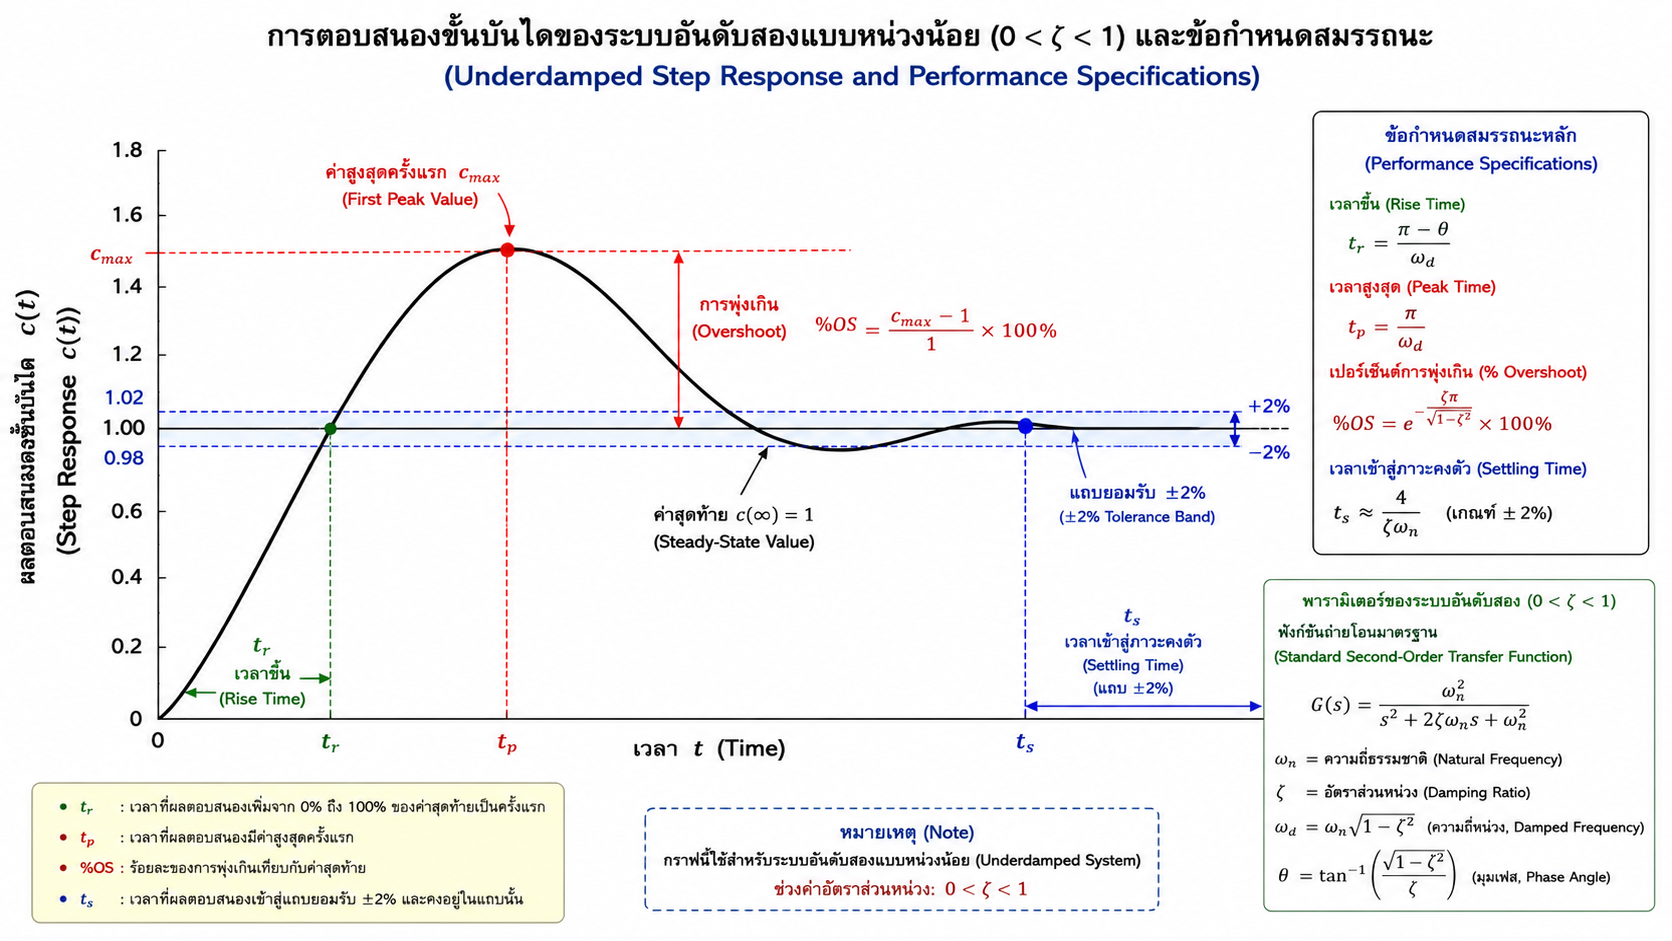
\includegraphics[width=0.8\textwidth]{images/chapter5/figure-04.png}
    \caption{กราฟผลตอบสนองอันดับสองแบบ Underdamped พร้อมระบุข้อกำหนดสมรรถนะ}
\end{figure}



\textbf{ตัวอย่างที่ 3 (เชิงวิเคราะห์): การคำนวณข้อกำหนดสมรรถนะ}

โจทย์: จากระบบในตัวอย่างที่ 2 ($\zeta=0.35$, $\omega_n=6$ rad/s, $\omega_d=5.62$ rad/s) จงคำนวณ $t_p$, $\%OS$, $t_s$ (เกณฑ์ 2\%) และ $t_r$ โดยประมาณ

\textit{ขั้นตอนที่ 1 วิเคราะห์ระบบ:} ใช้พารามิเตอร์ ζ, ωn, ωd ที่ได้จากตัวอย่างที่ 2

\textit{ขั้นตอนที่ 2 กำหนดตัวแปร:} ใช้สูตรข้อกำหนดสมรรถนะทั้งสี่

\textit{ขั้นตอนที่ 3 เลือกหลักการ:} สูตร $t_p=\pi/\omega_d$, $\%OS=e^{-\zeta\pi/\sqrt{1-\zeta^2}}\times100$, $t_s=4/(\zeta\omega_n)$, $t_r\approx1.8/\omega_n$

\textit{ขั้นตอนที่ 4–5 สร้างและจัดรูปสมการ:} แทนค่าพารามิเตอร์ลงในแต่ละสูตรโดยตรง

\textit{ขั้นตอนที่ 6–7 แทนค่าและคำนวณ:}

\[
t_p = \frac{\pi}{5.62} = 0.559 \text{ s}
\]

\[
\%OS = e^{-0.35\pi/\sqrt{1-0.1225}} \times 100 = e^{-1.174}\times100 = 30.9\%
\]

\[
t_s = \frac{4}{0.35\times6} = \frac{4}{2.1} = 1.90 \text{ s}
\]

\[
t_r \approx \frac{1.8}{6} = 0.30 \text{ s}
\]

\textit{ขั้นตอนที่ 8 ตรวจสอบความสมเหตุสมผล:} ค่า $t_r < t_p < t_s$ เป็นลำดับที่สมเหตุสมผล เพราะระบบต้องขึ้นถึงค่าสุดท้ายก่อน จึงจะแกว่งถึงจุดสูงสุด แล้วจึงค่อยสงบนิ่ง และ ζ=0.35 อยู่ในช่วงที่สูตรประมาณ $t_r$ ใช้ได้ดี (0.3–0.8)

\textit{ขั้นตอนที่ 9 แปลความหมาย:} ระบบนี้จะพุ่งเกินค่าสุดท้ายถึง 30.9\% ซึ่งค่อนข้างสูง และใช้เวลาเกือบ 2 วินาทีกว่าจะสงบนิ่งเข้าสู่ค่าคงตัว หากข้อกำหนดของงานต้องการ \%OS ที่ต่ำกว่านี้ จำเป็นต้องปรับค่า ζ ให้สูงขึ้น ดังแสดงในตัวอย่างถัดไป



\textbf{ตัวอย่างที่ 4 (ประยุกต์ใช้): การออกแบบค่าอัตราขยาย K ให้เป็นไปตามข้อกำหนดสมรรถนะ}

โจทย์: ระบบควบคุมความเร็วมอเตอร์มีฟังก์ชันถ่ายโอนวงเปิด $G(s)=\dfrac{K}{s(s+6)}$ ต่อแบบป้อนกลับหนึ่งหน่วย (Unity Feedback) ข้อกำหนดของงานต้องการ $\%OS \le 16\%$ และ $t_s \le 2$ วินาที (เกณฑ์ 2\%) โดยพิจารณาเฉพาะกรณีที่ระบบมีลักษณะ Underdamped จงหาช่วงค่า K ที่เป็นไปได้

\textit{ขั้นตอนที่ 1 วิเคราะห์ระบบ:} หาฟังก์ชันถ่ายโอนวงปิดก่อน

\[
T(s) = \frac{G(s)}{1+G(s)} = \frac{K}{s^2+6s+K}
\]

\textit{ขั้นตอนที่ 2 กำหนดตัวแปร:} เทียบกับรูปมาตรฐานได้ $\omega_n^2=K$ และ $2\zeta\omega_n=6 \Rightarrow \zeta\omega_n=3$ (ค่าคงที่ ไม่ขึ้นกับ K)

\textit{ขั้นตอนที่ 3 เลือกหลักการ:} ใช้สูตร \%OS หาค่า ζ ต่ำสุดที่ยอมรับได้ก่อน แล้วจึงหา ωn และ K

\textit{ขั้นตอนที่ 4–5 สร้างและจัดรูปสมการ:} จากสูตรผกผัน

\[
\zeta_{min} = \frac{-\ln(0.16)}{\sqrt{\pi^2+\ln^2(0.16)}}
\]

\textit{ขั้นตอนที่ 6 แทนค่า:} $\ln(0.16) = -1.833$

\[
\zeta_{min} = \frac{1.833}{\sqrt{9.870+3.358}} = \frac{1.833}{\sqrt{13.228}} = \frac{1.833}{3.637} = 0.504
\]

\textit{ขั้นตอนที่ 7 คำนวณ:} เนื่องจาก $\zeta\omega_n=3$ คงที่ ดังนั้น $\omega_n = 3/\zeta$ เมื่อ $\zeta \ge 0.504$ จะได้

\[
\omega_n \le \frac{3}{0.504} = 5.95 \text{ rad/s} \;\Rightarrow\; K=\omega_n^2 \le 35.4
\]

ตรวจสอบเงื่อนไข Underdamped ($\zeta<1$): ที่ $\zeta=1$ จะได้ $\omega_n=3$ rad/s หรือ $K=9$ ดังนั้นต้องมี $K>9$

ตรวจสอบ Settling Time: เนื่องจาก $\zeta\omega_n=3$ คงที่เสมอในระบบนี้ (ไม่ขึ้นกับ K) จะได้ $t_s=4/(\zeta\omega_n)=4/3=1.33$ วินาที ซึ่ง\textbf{น้อยกว่า 2 วินาทีเสมอ} ไม่ว่า K จะมีค่าใดในช่วง Underdamped

\textit{ขั้นตอนที่ 8 ตรวจสอบความสมเหตุสมผล:} ผลลัพธ์แสดงว่า Settling Time ของระบบนี้ถูกกำหนดตายตัวโดยตำแหน่งโพลที่ $s=-6$ ของระบบวงเปิด ซึ่งปรับด้วยค่า K เพียงอย่างเดียวไม่ได้ เป็นข้อจำกัดเชิงโครงสร้างของระบบที่ควรตระหนัก

\textit{ขั้นตอนที่ 9 แปลความหมาย:} ค่า K ที่ทำให้ระบบเป็นไปตามข้อกำหนดทั้งสองข้อ (โดยยังคง Underdamped) คือ \textbf{$9 < K \le 35.4$} โดย Settling Time จะเป็นไปตามข้อกำหนดโดยอัตโนมัติในช่วงนี้ หากต้องการปรับ Settling Time ให้เร็วขึ้นอีก จำเป็นต้องเปลี่ยนโครงสร้างของตัวควบคุม ไม่ใช่ปรับเพียงค่า K


\subsubsection{7.5 ความผิดพลาดคงตัว (Steady-State Error)}

นอกจากพฤติกรรมชั่วครู่แล้ว วิศวกรยังต้องพิจารณาว่าเมื่อเวลาผ่านไปนานพอ ผลตอบสนองของระบบจะติดตามสัญญาณอ้างอิงได้แม่นยำเพียงใด ผลต่างนี้เรียกว่า \textbf{ความผิดพลาดคงตัว (Steady-State Error, $e_{ss}$)}

\textbf{การหา ess ด้วยทฤษฎีบทค่าสุดท้าย}

สำหรับระบบป้อนกลับหนึ่งหน่วย (Unity Feedback) สัญญาณความผิดพลาดคือ

\[
E(s) = \frac{R(s)}{1+G(s)}
\]

ใช้ทฤษฎีบทค่าสุดท้าย (Final Value Theorem) จะได้

\[
e_{ss} = \lim_{t\to\infty} e(t) = \lim_{s\to0} sE(s) = \lim_{s\to0}\frac{sR(s)}{1+G(s)}
\]

\textbf{System Type}

นิยาม \textbf{ชนิดของระบบ (System Type)} คือจำนวนโพลของฟังก์ชันถ่ายโอนวงเปิด $G(s)$ ที่ตำแหน่ง $s=0$ (จำนวนตัวรวมสัญญาณหรือ Integrator ในวงเปิด) เขียนแทนด้วย $n$ ในรูปทั่วไป

\[
G(s) = \frac{K\prod(s+z_i)}{s^n\prod(s+p_j)}
\]

\textbf{ข้อควรระวัง:} System Type แตกต่างจากอันดับของระบบ (System Order) โดยสิ้นเชิง อันดับของระบบคือจำนวนโพลทั้งหมดของฟังก์ชันถ่ายโอนวงปิด ในขณะที่ System Type นับเฉพาะโพลที่ $s=0$ ของวงเปิดเท่านั้น

\textbf{ค่าคงที่ความผิดพลาด (Static Error Constants)}

\begin{table}[htbp]
    \centering
    \begin{tabular}{llll}
        \hline
        \textbf{ชื่อ} & \textbf{นิยาม} & \textbf{สัญญาณอ้างอิง} & \textbf{$e_{ss}$} \\
        \hline
        Position Error Constant & $K_p = \lim\limits_{s\to0} G(s)$ & ขั้นบันได $R(s)=1/s$ & $e_{ss} = \dfrac{1}{1+K_p}$ \\
        Velocity Error Constant & $K_v = \lim\limits_{s\to0} sG(s)$ & ทางลาด $R(s)=1/s^2$ & $e_{ss} = \dfrac{1}{K_v}$ \\
        Acceleration Error Constant & $K_a = \lim\limits_{s\to0} s^2G(s)$ & พาราโบลา $R(s)=1/s^3$ & $e_{ss} = \dfrac{1}{K_a}$ \\
        \hline
    \end{tabular}
\end{table}

\textbf{ความสัมพันธ์ระหว่าง System Type กับ ess}

\begin{table}[htbp]
    \centering
    \begin{tabular}{lrrr}
        \hline
        \textbf{System Type} & \textbf{$e_{ss}$ ต่อสัญญาณขั้นบันได} & \textbf{$e_{ss}$ ต่อสัญญาณทางลาด} & \textbf{$e_{ss}$ ต่อสัญญาณพาราโบลา} \\
        \hline
        Type 0 & จำกัด $= \dfrac{1}{1+K_p}$ & $\infty$ & $\infty$ \\
        Type 1 & $0$ & จำกัด $= \dfrac{1}{K_v}$ & $\infty$ \\
        Type 2 & $0$ & $0$ & จำกัด $= \dfrac{1}{K_a}$ \\
        \hline
    \end{tabular}
\end{table}

ตารางนี้แสดงหลักการสำคัญว่า \textbf{ระบบต้องมีตัวรวมสัญญาณอย่างน้อยเท่ากับดีกรีของสัญญาณอ้างอิง บวกหนึ่ง จึงจะติดตามสัญญาณนั้นได้โดยไม่มีความผิดพลาดคงตัว} เช่น การติดตามสัญญาณทางลาดโดยไม่มีความผิดพลาดคงตัวเลยต้องใช้ระบบ Type 2 ขึ้นไป



\textbf{ตัวอย่างที่ 5 (ประยุกต์ใช้): การหาชนิดของระบบและความผิดพลาดคงตัว}

โจทย์: ระบบป้อนกลับหนึ่งหน่วยมีฟังก์ชันถ่ายโอนวงเปิด $G(s)=\dfrac{20}{s(s+5)}$ จงหาชนิดของระบบ ค่า $K_p$, $K_v$, $K_a$ และความผิดพลาดคงตัวเมื่อป้อนสัญญาณทางลาดหนึ่งหน่วย $r(t)=t$

\textit{ขั้นตอนที่ 1 วิเคราะห์ระบบ:} $G(s)$ มีตัวประกอบ $s$ หนึ่งตัวในตัวส่วน จึงมีโพลที่ $s=0$ จำนวน 1 ตัว

\textit{ขั้นตอนที่ 2 กำหนดตัวแปร:} System Type $= 1$

\textit{ขั้นตอนที่ 3 เลือกหลักการ:} ใช้นิยาม $K_p$, $K_v$, $K_a$ ตามตาราง

\textit{ขั้นตอนที่ 4–5 สร้างและจัดรูปสมการ:}

\[
K_p = \lim_{s\to0} \frac{20}{s(s+5)} \to \infty \quad (\text{เนื่องจากตัวส่วนมี } s)
\]

\[
K_v = \lim_{s\to0} s\cdot\frac{20}{s(s+5)} = \lim_{s\to0}\frac{20}{s+5}
\]

\[
K_a = \lim_{s\to0} s^2\cdot\frac{20}{s(s+5)} = \lim_{s\to0}\frac{20s}{s+5}
\]

\textit{ขั้นตอนที่ 6–7 แทนค่าและคำนวณ:}

\[
K_v = \frac{20}{5} = 4, \qquad K_a = \frac{20\times0}{5} = 0
\]

ดังนั้น $e_{ss}(\text{step}) = \dfrac{1}{1+K_p} = 0$, $\quad e_{ss}(\text{ramp}) = \dfrac{1}{K_v} = \dfrac{1}{4} = 0.25$, $\quad e_{ss}(\text{parabola}) = \dfrac{1}{K_a} \to \infty$

\textit{ขั้นตอนที่ 8 ตรวจสอบความสมเหตุสมผล:} ผลลัพธ์สอดคล้องกับตารางในหัวข้อนี้พอดี เพราะระบบเป็น Type 1: $e_{ss}(\text{step})=0$, $e_{ss}(\text{ramp})$ มีค่าจำกัด, $e_{ss}(\text{parabola})=\infty$

\textit{ขั้นตอนที่ 9 แปลความหมาย:} เมื่อสั่งให้ระบบติดตามสัญญาณทางลาดหนึ่งหน่วย (เช่น ความเร็วอ้างอิงคงที่) ผลตอบสนองที่สภาวะคงตัวจะตามหลังสัญญาณอ้างอิงอยู่คงที่ 0.25 หน่วยเสมอ ซึ่งเป็นความผิดพลาดเชิงตำแหน่งที่ยอมรับได้หรือไม่ขึ้นอยู่กับข้อกำหนดของงานนั้น ๆ หากต้องการลดค่านี้ วิศวกรสามารถเพิ่มอัตราขยายวงเปิด (เพิ่มค่าคงที่ 20 ให้สูงขึ้น) เพื่อเพิ่ม $K_v$



\subsubsection{7.6 การจำลองผลตอบสนองด้วย MATLAB}

ซอฟต์แวร์ MATLAB พร้อม Control System Toolbox ช่วยให้วิเคราะห์ผลตอบสนองชั่วครู่และคำนวณข้อกำหนดสมรรถนะได้อย่างรวดเร็ว โดยไม่ต้องคำนวณด้วยมือทุกขั้นตอน ซึ่งมีประโยชน์อย่างยิ่งเมื่อต้องเปรียบเทียบหลายกรณีพร้อมกัน

\textbf{วัตถุประสงค์การใช้ซอฟต์แวร์:} สร้างฟังก์ชันถ่ายโอน พล็อตผลตอบสนองต่อสัญญาณขั้นบันได และคำนวณข้อกำหนดสมรรถนะโดยอัตโนมัติ เพื่อตรวจสอบผลการคำนวณด้วยมือและใช้เปรียบเทียบกับผลการทดลองจริงในกิจกรรมปฏิบัติการ

\begin{verbatim}
% กำหนดพารามิเตอร์ระบบอันดับสอง (ใช้ค่าจากตัวอย่างที่ 2-3)
zeta = 0.35;
wn = 6;

% สร้างฟังก์ชันถ่ายโอนในรูปมาตรฐาน
num = wn^2;
den = [1, 2*zeta*wn, wn^2];
sys = tf(num, den);

% พล็อตผลตอบสนองต่อสัญญาณขั้นบันได
figure;
step(sys);
grid on;
title('Step Response, \zeta = 0.35, \omega_n = 6 rad/s');

% คำนวณข้อกำหนดสมรรถนะโดยอัตโนมัติ
info = stepinfo(sys);
disp(info)
\end{verbatim}

คำสั่ง \texttt{stepinfo(sys)} จะคืนค่าโครงสร้างข้อมูลที่มีฟิลด์สำคัญ ได้แก่ \texttt{RiseTime}, \texttt{SettlingTime}, \texttt{Overshoot} (มีหน่วยเป็นเปอร์เซ็นต์อยู่แล้ว), \texttt{Peak} และ \texttt{PeakTime} ซึ่งควรมีค่าใกล้เคียงกับที่คำนวณด้วยมือในตัวอย่างที่ 3 (ความแตกต่างเล็กน้อยเกิดจาก MATLAB ใช้เกณฑ์ Settling Time เริ่มต้นที่ 2\% และคำนวณ Rise Time แบบ 0–100\% อย่างแม่นยำ ไม่ใช่ค่าประมาณ)

หากต้องการเปรียบเทียบผลตอบสนองสำหรับหลายค่า ζ พร้อมกันในกราฟเดียว (เช่นเดียวกับรูปที่ 3) สามารถวนลูปและใช้ \texttt{hold on} ได้ดังนี้

\begin{verbatim}
% เปรียบเทียบผลตอบสนองสำหรับหลายค่า zeta ที่ wn คงที่
wn = 6;
zeta_values = [0.2, 0.5, 0.7, 1.0, 2.0];

figure; hold on;
for z = zeta_values
    sys = tf(wn^2, [1, 2*z*wn, wn^2]);
    step(sys);
end
legend('\zeta=0.2', '\zeta=0.5', '\zeta=0.7', '\zeta=1.0', '\zeta=2.0');
grid on;
title('Step Response Comparison for Different Damping Ratios');
\end{verbatim}

\textbf{ค่าที่ผู้เรียนต้องปรับ:} \texttt{zeta}, \texttt{wn} ให้ตรงกับระบบที่กำลังวิเคราะห์ในแต่ละกรณี

\textbf{ผลลัพธ์ที่ควรสังเกต:} เมื่อ ζ เพิ่มขึ้น เส้นกราฟควรแกว่งน้อยลงและค่า Overshoot ที่ MATLAB คำนวณควรลดลงตามสูตรในหัวข้อ 7.4

\textbf{ข้อผิดพลาดที่พบบ่อย:} การลืมกำหนดลำดับสัมประสิทธิ์ในตัวแปร \texttt{den} ให้ถูกต้อง (ต้องเรียงจากดีกรีสูงไปต่ำ) และการสับสนระหว่างหน่วย Overshoot ที่ MATLAB แสดงเป็นเปอร์เซ็นต์อยู่แล้วกับสัดส่วน (Fraction) ที่บางครั้งใช้ในการคำนวณด้วยมือ

\textbf{ข้อจำกัด:} \texttt{stepinfo} ใช้เกณฑ์ Settling Time เริ่มต้นที่ 2\% และ Rise Time แบบ 0–100\% หากต้องการเปลี่ยนเกณฑ์ต้องระบุพารามิเตอร์เพิ่มเติม เช่น \texttt{stepinfo(sys,'SettlingTimeThreshold',0.05)} สำหรับเกณฑ์ 5\% ทั้งนี้คำสั่งและผลลัพธ์อาจแตกต่างกันเล็กน้อยระหว่างเวอร์ชันของ MATLAB จึงควรตรวจสอบกับเอกสารของเวอร์ชันที่ใช้งานจริง



\subsection{8. ความเข้าใจผิดที่พบบ่อย}

\textbf{ความเข้าใจผิดที่ 1:} ค่าคงเวลา τ คือเวลาที่ระบบเข้าสู่สภาวะคงตัวอย่างสมบูรณ์
\textbf{แนวคิดที่ถูกต้อง:} τ เป็นเพียงจุดอ้างอิงที่ระบบตอบสนองได้ 63.2\% ของค่าสุดท้ายเท่านั้น ระบบต้องใช้เวลาประมาณ 4τ ถึง 5τ จึงจะถือว่าเข้าสู่สภาวะคงตัวตามเกณฑ์ที่ยอมรับทั่วไป (2\% หรือ 1\%)

\textbf{ความเข้าใจผิดที่ 2:} Settling Time คำนวณด้วยเกณฑ์เดียวเสมอ
\textbf{แนวคิดที่ถูกต้อง:} ในทางปฏิบัติอาจใช้เกณฑ์ 2\% หรือ 5\% ขึ้นกับมาตรฐานหรือข้อตกลงของงานนั้น ๆ ผลลัพธ์ที่ได้จากสูตร $4/(\zeta\omega_n)$ และ $3/(\zeta\omega_n)$ จึงต่างกัน ต้องระบุเกณฑ์ที่ใช้กำกับไว้เสมอเพื่อไม่ให้สื่อสารคลาดเคลื่อน

\textbf{ความเข้าใจผิดที่ 3:} Percent Overshoot ขึ้นอยู่กับขนาดของสัญญาณเข้าหรือค่าสุดท้ายของผลตอบสนอง
\textbf{แนวคิดที่ถูกต้อง:} สำหรับระบบเชิงเส้นอันดับสองมาตรฐาน \%OS เป็นค่าสัดส่วน (Normalized) ที่ขึ้นอยู่กับ ζ เพียงตัวแปรเดียวเท่านั้น ไม่ว่าขนาดสัญญาณขั้นบันไดจะเป็นเท่าใด \%OS จะยังคงเท่าเดิมตราบใดที่ ζ ไม่เปลี่ยน

\textbf{ความเข้าใจผิดที่ 4:} ωn คือความถี่ที่สังเกตเห็นการแกว่งจริงบนกราฟหรือออสซิลโลสโคป
\textbf{แนวคิดที่ถูกต้อง:} ความถี่ที่วัดได้จากคาบการแกว่งจริงคือ ωd (Damped Frequency) ไม่ใช่ ωn โดย $\omega_d=\omega_n\sqrt{1-\zeta^2}$ เสมอสำหรับกรณี Underdamped ทั้งสองค่าจะเท่ากันก็ต่อเมื่อ ζ=0 เท่านั้น ซึ่งไม่เกิดขึ้นในระบบจริงที่มีการสูญเสียพลังงาน

\textbf{ความเข้าใจผิดที่ 5:} "อันดับของระบบ" (System Order) และ "ชนิดของระบบ" (System Type) มีความหมายเดียวกัน
\textbf{แนวคิดที่ถูกต้อง:} อันดับของระบบคือดีกรีของพหุนามตัวส่วนของฟังก์ชันถ่ายโอนวงปิด (จำนวนโพลทั้งหมด) ในขณะที่ System Type นับเฉพาะจำนวนโพลของฟังก์ชันถ่ายโอน\textbf{วงเปิด}ที่ตำแหน่ง $s=0$ เท่านั้น ระบบอันดับสองอาจเป็น Type 0, 1 หรือ 2 ก็ได้ ขึ้นกับโครงสร้างของ G(s)

\textbf{ความเข้าใจผิดที่ 6:} System Type ที่สูงกว่าย่อมดีกว่าเสมอ
\textbf{แนวคิดที่ถูกต้อง:} การเพิ่มตัวรวมสัญญาณ (Integrator) เพื่อยกระดับ System Type ช่วยลดความผิดพลาดคงตัวก็จริง แต่มักทำให้เสถียรภาพของระบบลดลงและการออกแบบซับซ้อนขึ้น การเลือก System Type ต้องพิจารณาจากข้อกำหนดของงานจริง ไม่ใช่เลือกให้สูงที่สุดเสมอไป



\subsection{9. การประยุกต์ใช้ในงานจริง}

\textbf{ระบบควบคุมความเร็วมอเตอร์ไฟฟ้ากระแสตรง (DC Motor Speed Control):} วิศวกรต้องกำหนด Rise Time ให้สั้นพอสำหรับการตอบสนองที่รวดเร็ว ขณะเดียวกันต้องจำกัด \%OS เพื่อไม่ให้ความเร็วพุ่งเกินจนสร้างความเสียหายต่อกลไกขับเคลื่อนหรือชิ้นงานที่ต่อพ่วง

\textbf{ระบบลิฟต์โดยสาร (Elevator Position Control):} Settling Time ที่สั้นเกินไปอาจทำให้ลิฟต์เร่ง-เบรกกะทันหันจนผู้โดยสารไม่สบายตัว ในขณะที่ \%OS ต้องควบคุมให้ต่ำมากหรือเป็นศูนย์ เพื่อป้องกันไม่ให้ลิฟต์หยุดเลยตำแหน่งชั้นที่กำหนด

\textbf{ระบบควบคุมอุณหภูมิเตาอบอุตสาหกรรม (Industrial Oven Temperature Control):} เนื่องจากระบบความร้อนมักมีค่าคงเวลาสูง (ตอบสนองช้า) การออกแบบต้องคำนึงถึง Settling Time ที่ยาวนานและความผิดพลาดคงตัวที่อาจเกิดจากการสูญเสียความร้อนสู่สิ่งแวดล้อม

\textbf{ระบบกันสะเทือนรถยนต์ (Automotive Suspension System):} อัตราส่วนหน่วง ζ ของระบบกันสะเทือนถูกออกแบบอย่างระมัดระวังเพื่อสมดุลระหว่างความนุ่มนวล (ζ ต่ำ แกว่งได้) กับความมั่นคงในการควบคุมรถ (ζ สูง ไม่แกว่ง) เป็นตัวอย่างที่ดีของการแลกเปลี่ยน (Trade-off) ระหว่าง \%OS กับ Settling Time

\textbf{ระบบควบคุมการทรงตัวของโดรนหรือหุ่นยนต์ (Drone/Robot Attitude Control):} \%OS ที่สูงเกินไปในมุมเอียงของโดรนอาจนำไปสู่การสูญเสียการทรงตัวหรือชนสิ่งกีดขวาง ในขณะที่ Rise Time ต้องเร็วพอเพื่อให้ระบบตอบสนองต่อการรบกวนจากลมหรือแรงภายนอกได้ทันเวลา

\newpage

\subsection{10. กิจกรรมปฏิบัติการ}

\subsubsection{กิจกรรมปฏิบัติการที่ 1: การวัดผลตอบสนองชั่วครู่ของวงจร RC (ระบบอันดับหนึ่ง)}

\textbf{1. วัตถุประสงค์}
เมื่อเสร็จสิ้นกิจกรรมนี้ ผู้เรียนสามารถต่อวงจร RC วัดผลตอบสนองต่อสัญญาณขั้นบันไดด้วยออสซิลโลสโคป หาค่าคงเวลา τ จากข้อมูลที่วัดได้จริง และเปรียบเทียบกับค่าที่คำนวณจากทฤษฎี $\tau=RC$

\textbf{2. หลักการและทฤษฎีที่เกี่ยวข้อง}\par\noindent
วงจร RC อนุกรมที่วัดแรงดันคร่อมตัวเก็บประจุมีฟังก์ชันถ่ายโอน $V_C(s)/V_{in}(s) = 1/(RCs+1)$ ซึ่งเป็นระบบอันดับหนึ่งมาตรฐานตามหัวข้อ 7.1 โดยค่าคงเวลาทางทฤษฎีคือ $\tau=RC$

\textbf{3. อุปกรณ์ เครื่องมือ และซอฟต์แวร์}

\begin{itemize}
    \item เครื่องกำเนิดสัญญาณ (Function Generator) ตั้งค่าสัญญาณคลื่นสี่เหลี่ยม (Square Wave) 1 เครื่อง
    \item ออสซิลโลสโคป 1 เครื่อง พร้อมสายโพรบ 2 ชุด
    \item ตัวต้านทาน (Resistor) ค่าต่าง ๆ อย่างน้อย 3 ค่า
    \item ตัวเก็บประจุ (Capacitor) ค่าต่าง ๆ อย่างน้อย 2 ค่า
    \item เบรดบอร์ดและสายเชื่อมต่อ
    \item มัลติมิเตอร์ 1 เครื่อง (สำหรับตรวจสอบค่า R, C จริง)
\end{itemize}

\textbf{4. แผนภาพหรือวงจร}

% [รูปที่ 5: วงจร RC อนุกรมสำหรับกิจกรรมปฏิบัติการที่ 1]
% ประเภทภาพ: Experimental Setup
% ตำแหน่งที่แนะนำ: หัวข้อ 10 กิจกรรมปฏิบัติการที่ 1 ส่วนที่ 4
% วัตถุประสงค์การเรียนรู้: ให้ผู้เรียนเข้าใจการต่อวงจรจริงและตำแหน่งการวัดแรงดันด้วยออสซิลโลสโคป
% คำอธิบายภาพ: วงจรอนุกรมประกอบด้วยเครื่องกำเนิดสัญญาณคลื่นสี่เหลี่ยมต่อผ่านตัวต้านทาน R ไปยังตัวเก็บประจุ C ที่ต่อลงกราวด์ ปลายสายโพรบช่อง 1 ของออสซิลโลสโคปวัดสัญญาณเข้า (Vin) ปลายสายโพรบช่อง 2 วัดแรงดันคร่อม C (Vc)
% องค์ประกอบที่ต้องมี: สัญลักษณ์เครื่องกำเนิดสัญญาณ, ตัวต้านทาน R, ตัวเก็บประจุ C, จุดกราวด์, ตำแหน่งโพรบ CH1 และ CH2
% ข้อความหรือป้ายกำกับ: "Vin", "R", "C", "Vc", "CH1", "CH2", "GND"
% ภาษาของป้ายกำกับ: ไทยและอังกฤษ
% สัดส่วนภาพ: 4:3
% Image Generation Prompt: Simple series RC circuit schematic diagram, function generator connected through a resistor to a capacitor to ground, oscilloscope probes labeled CH1 at input and CH2 across the capacitor, clean technical schematic style, black lines on white background
% Alt Text: แผนภาพวงจร RC อนุกรมพร้อมตำแหน่งการวัดด้วยออสซิลโลสโคปสำหรับกิจกรรมปฏิบัติการที่ 1

\begin{figure}[htbp]
    \centering
    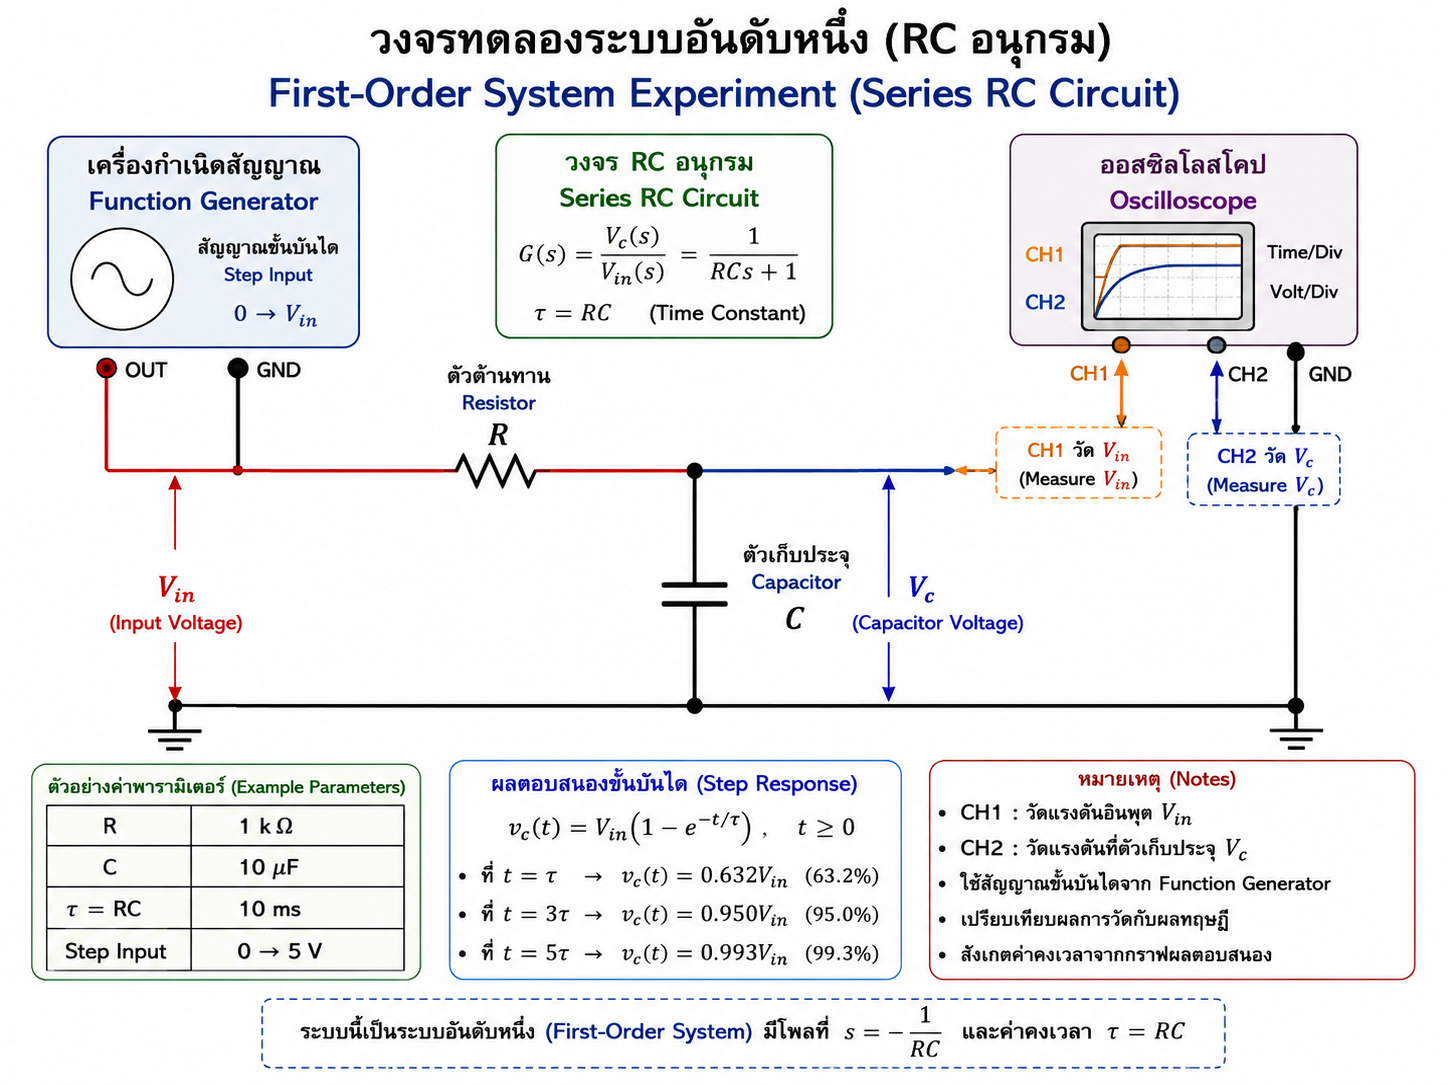
\includegraphics[width=0.8\textwidth]{images/chapter5/figure-05.png}
    \caption{วงจร RC อนุกรมสำหรับกิจกรรมปฏิบัติการที่ 1}
\end{figure}

\textbf{5. ข้อควรระวังด้านความปลอดภัย}

\begin{itemize}
    \item ใช้แรงดันจากเครื่องกำเนิดสัญญาณไม่เกิน 10–15 V เพื่อความปลอดภัยและป้องกันความเสียหายต่ออุปกรณ์
    \item ตรวจสอบขั้วของตัวเก็บประจุแบบมีขั้ว (Electrolytic) ก่อนต่อวงจรทุกครั้ง
    \item ปิดเครื่องกำเนิดสัญญาณก่อนเปลี่ยนค่าตัวต้านทานหรือตัวเก็บประจุทุกครั้ง
    \item ต่อกราวด์ของออสซิลโลสโคปและเครื่องกำเนิดสัญญาณเข้าจุดเดียวกันเสมอ
\end{itemize}

\textbf{6. ขั้นตอนการปฏิบัติ}

\begin{enumerate}
    \item คำนวณค่า τ ทางทฤษฎีล่วงหน้าจากค่า R และ C ที่จะใช้ในแต่ละชุดการทดลอง
    \item ตั้งความถี่ของสัญญาณคลื่นสี่เหลี่ยมให้มีคาบมากกว่า $10\tau$ เพื่อให้เห็นผลตอบสนองครบสมบูรณ์ในแต่ละครึ่งคาบ
    \item ต่อวงจรตามรูปที่ 5 ด้วยค่า R และ C ชุดแรก
    \item ปรับออสซิลโลสโคปให้เห็นสัญญาณ Vin และ Vc พร้อมกันบนหน้าจอ
    \item ใช้เคอร์เซอร์ของออสซิลโลสโคปวัดเวลาที่ Vc มีค่าถึง 63.2\% ของค่าสุดท้าย บันทึกเป็น τ ที่วัดได้
    \item วัดเวลาที่ Vc ถึง 90\% และ 95\% เพิ่มเติมเพื่อตรวจสอบความสอดคล้องกับทฤษฎี
    \item เปลี่ยนค่า R หรือ C ตามชุดข้อมูลที่กำหนด แล้วทำซ้ำขั้นตอนที่ 4–6 จนครบ 3 ชุด
\end{enumerate}

\textbf{7. ตารางบันทึกผล}

\begin{table}[htbp]
    \centering
    \begin{tabular}{llllll}
        \hline
        \textbf{ชุดที่} & \textbf{R (Ω)} & \textbf{C (μF)} & \textbf{τ ทฤษฎี = RC (ms)} & \textbf{τ วัดได้ (ms)} & \textbf{\%ความคลาดเคลื่อน} \\
        \hline
        1 &  &  &  &  &  \\
        2 &  &  &  &  &  \\
        3 &  &  &  &  &  \\
        \hline
    \end{tabular}
\end{table}

\textbf{8. การคำนวณและวิเคราะห์ผล}

คำนวณ \%ความคลาดเคลื่อนจาก $\left|\dfrac{\tau_{\text{ทฤษฎี}}-\tau_{\text{วัดได้}}}{\tau_{\text{ทฤษฎี}}}\right|\times100$ และวิเคราะห์ว่าความคลาดเคลื่อนมีแนวโน้มเพิ่มขึ้นหรือลดลงเมื่อค่า R หรือ C เปลี่ยนแปลงหรือไม่

\textbf{9. การเปรียบเทียบผลจริงกับทฤษฎีหรือแบบจำลอง}

นำค่า τ ที่วัดได้มาพล็อตกราฟ $V_C(t)$ เปรียบเทียบกับกราฟทฤษฎีที่ได้จาก MATLAB (หัวข้อ 7.6) โดยใช้ค่า R, C จริงที่วัดด้วยมัลติมิเตอร์

\textbf{10. คำถามหลังการทดลอง}

\begin{itemize}
    \item ค่า τ ที่วัดได้สอดคล้องกับค่าทางทฤษฎีหรือไม่ หากมีความคลาดเคลื่อน สาเหตุที่เป็นไปได้คืออะไร
    \item หากเพิ่มค่า R เป็นสองเท่าโดยคงค่า C เดิม τ ที่วัดได้ควรเปลี่ยนแปลงอย่างไร ผลการทดลองสอดคล้องกับที่คาดการณ์หรือไม่
    \item เหตุใดจึงต้องตั้งคาบของสัญญาณคลื่นสี่เหลี่ยมให้มากกว่า $10\tau$
\end{itemize}

\textbf{11. เกณฑ์การประเมิน}

ความถูกต้องของการต่อวงจรและการตั้งค่าเครื่องมือ, ความแม่นยำในการอ่านค่าจากออสซิลโลสโคป, ความครบถ้วนของการบันทึกผล, คุณภาพของการวิเคราะห์เปรียบเทียบทฤษฎีกับผลจริง, การตอบคำถามหลังการทดลอง และการปฏิบัติตามข้อควรระวังด้านความปลอดภัย



\subsubsection{กิจกรรมปฏิบัติการที่ 2: การวัดผลตอบสนองชั่วครู่ของวงจร RLC (ระบบอันดับสอง) และการเปรียบเทียบกับ MATLAB}

\textbf{1. วัตถุประสงค์}
เมื่อเสร็จสิ้นกิจกรรมนี้ ผู้เรียนสามารถต่อวงจร RLC อนุกรม ปรับค่า R เพื่อให้เกิดการตอบสนองแบบ Underdamped, Critically Damped และ Overdamped อ่านค่า $t_r$, $t_p$, $\%OS$, $t_s$ จากออสซิลโลสโคป และเปรียบเทียบกับผลการจำลองด้วย MATLAB

\textbf{2. หลักการและทฤษฎีที่เกี่ยวข้อง}
วงจร RLC อนุกรมที่วัดแรงดันคร่อมตัวเก็บประจุมีฟังก์ชันถ่ายโอน

\[
\frac{V_C(s)}{V_{in}(s)} = \frac{1/LC}{s^2+(R/L)s+1/LC}
\]

เทียบกับรูปมาตรฐานในหัวข้อ 7.2 จะได้

\[
\omega_n = \frac{1}{\sqrt{LC}}, \qquad \zeta = \frac{R}{2}\sqrt{\frac{C}{L}}
\]

สังเกตว่า ζ แปรผันตรงกับ R โดยตรง การปรับค่า R จึงเป็นวิธีที่สะดวกที่สุดในการเปลี่ยนลักษณะการหน่วงของวงจรโดยไม่ต้องเปลี่ยน L หรือ C

\textbf{3. อุปกรณ์ เครื่องมือ และซอฟต์แวร์}

\begin{itemize}
    \item เครื่องกำเนิดสัญญาณคลื่นสี่เหลี่ยม 1 เครื่อง
    \item ออสซิลโลสโคป 1 เครื่อง พร้อมสายโพรบ 2 ชุด
    \item กล่องตัวต้านทานปรับค่าได้ (Decade Resistance Box) หรือชุดตัวต้านทานหลายค่า
    \item ตัวเหนี่ยวนำ (Inductor) L = 10 mH จำนวน 1 ตัว
    \item ตัวเก็บประจุ (Capacitor) C = 1 μF จำนวน 1 ตัว
    \item เบรดบอร์ดและสายเชื่อมต่อ
    \item คอมพิวเตอร์ที่ติดตั้ง MATLAB
\end{itemize}

\textbf{4. แผนภาพหรือวงจร}

% [รูปที่ 6: วงจร RLC อนุกรมสำหรับกิจกรรมปฏิบัติการที่ 2]
% ประเภทภาพ: Experimental Setup
% ตำแหน่งที่แนะนำ: หัวข้อ 10 กิจกรรมปฏิบัติการที่ 2 ส่วนที่ 4
% วัตถุประสงค์การเรียนรู้: ให้ผู้เรียนเข้าใจการต่อวงจร RLC อนุกรมและตำแหน่งการวัดที่สอดคล้องกับฟังก์ชันถ่ายโอนอันดับสอง
% คำอธิบายภาพ: วงจรอนุกรมประกอบด้วยเครื่องกำเนิดสัญญาณคลื่นสี่เหลี่ยมต่อผ่านตัวต้านทาน R ตัวเหนี่ยวนำ L และตัวเก็บประจุ C ตามลำดับ ลงกราวด์ ปลายสายโพรบช่อง 1 วัดสัญญาณเข้า ปลายสายโพรบช่อง 2 วัดแรงดันคร่อม C
% องค์ประกอบที่ต้องมี: สัญลักษณ์เครื่องกำเนิดสัญญาณ, R, L, C, จุดกราวด์, ตำแหน่งโพรบ CH1 และ CH2
% ข้อความหรือป้ายกำกับ: "Vin", "R", "L", "C", "Vc", "CH1", "CH2", "GND"
% ภาษาของป้ายกำกับ: ไทยและอังกฤษ
% สัดส่วนภาพ: 4:3
% Image Generation Prompt: Simple series RLC circuit schematic diagram, function generator connected through a resistor, inductor and capacitor in series to ground, oscilloscope probes labeled CH1 at input and CH2 across the capacitor, clean technical schematic style, black lines on white background
% Alt Text: แผนภาพวงจร RLC อนุกรมพร้อมตำแหน่งการวัดด้วยออสซิลโลสโคปสำหรับกิจกรรมปฏิบัติการที่ 2

\begin{figure}[htbp]
    \centering
    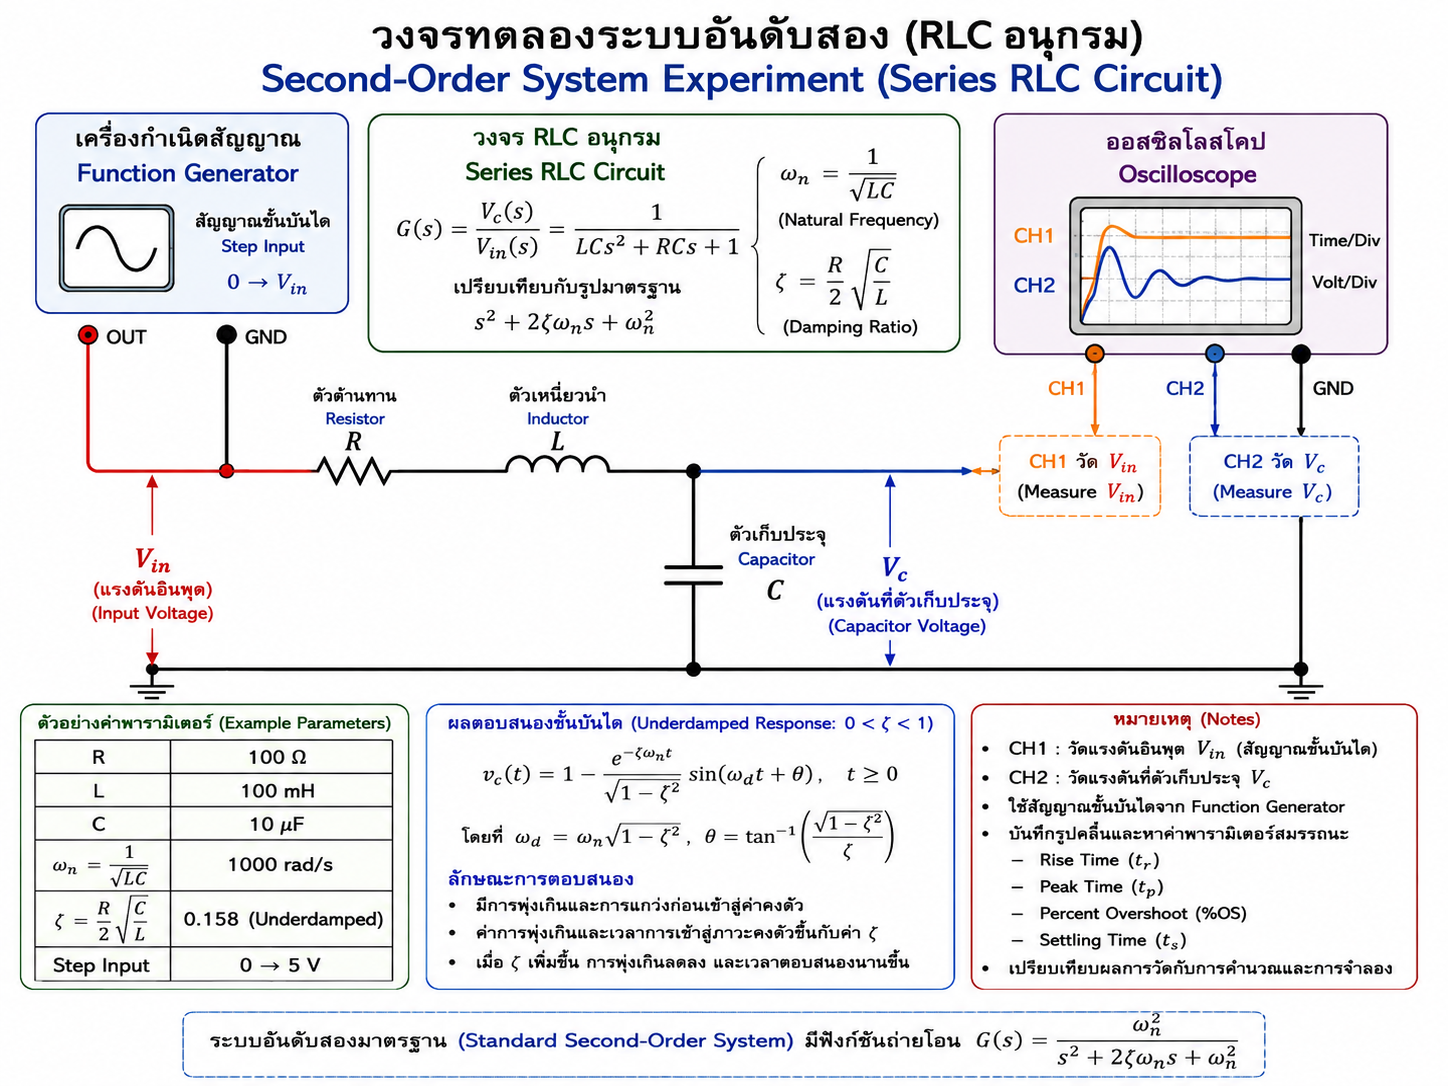
\includegraphics[width=0.8\textwidth]{images/chapter5/figure-06.png}
    \caption{วงจร RLC อนุกรมสำหรับกิจกรรมปฏิบัติการที่ 2}
\end{figure}

\textbf{5. ข้อควรระวังด้านความปลอดภัย}

\begin{itemize}
    \item ตรวจสอบพิกัดกระแสของตัวเหนี่ยวนำก่อนใช้งาน ไม่ให้เกินพิกัดที่ระบุ
    \item ระมัดระวังแรงดันเกิน (Voltage Spike) ที่อาจเกิดขึ้นชั่วขณะเมื่อกระแสผ่านตัวเหนี่ยวนำเปลี่ยนแปลงอย่างรวดเร็ว
    \item ใช้แรงดันจากเครื่องกำเนิดสัญญาณในระดับต่ำ (ไม่เกิน 10–15 V) ตลอดการทดลอง
    \item ต่อกราวด์ของอุปกรณ์ทุกชิ้นเข้าจุดเดียวกันเพื่อลดสัญญาณรบกวน
\end{itemize}

\textbf{6. ขั้นตอนการปฏิบัติ}

\begin{enumerate}
    \item คำนวณค่า $\omega_n=1/\sqrt{LC}$ จาก L=10 mH, C=1 μF ล่วงหน้า
    \item คำนวณค่า R ที่ต้องใช้เพื่อให้ได้ ζ เป้าหมาย 3 ค่า เช่น ζ≈0.3 (Underdamped), ζ=1 (Critically Damped) และ ζ≈2 (Overdamped) จากสูตร $R=2\zeta\sqrt{L/C}$
    \item ต่อวงจรตามรูปที่ 6 ด้วยค่า R ชุดแรก (Underdamped) ตั้งความถี่สัญญาณคลื่นสี่เหลี่ยมให้คาบมากกว่า $10\times t_s$ โดยประมาณ
    \item อ่านค่า $t_r$, $t_p$, $\%OS$, $t_s$ จากหน้าจอออสซิลโลสโคปโดยใช้เคอร์เซอร์วัดเวลาและแรงดัน บันทึกผล
    \item เปลี่ยนค่า R เป็นชุดถัดไป (Critically Damped และ Overdamped) แล้วทำซ้ำขั้นตอนที่ 4 สังเกตการหายไปของการแกว่ง
    \item ในโปรแกรม MATLAB สร้างฟังก์ชันถ่ายโอนด้วยค่า ωn, ζ ที่คำนวณได้ในแต่ละกรณี ใช้คำสั่ง \texttt{step()} และ \texttt{stepinfo()} ตามหัวข้อ 7.6 เพื่อหาค่าทฤษฎี
    \item เปรียบเทียบค่าที่วัดได้จริงกับค่าทฤษฎีจาก MATLAB ในตารางบันทึกผล
\end{enumerate}

\textbf{7. ตารางบันทึกผล}

\begin{table}[htbp]
    \centering
    \small
    \begin{tabularx}{\textwidth}{@{}>{\raggedright\arraybackslash}p{0.14\textwidth}*{7}{>{\centering\arraybackslash}X}@{}}
        \hline
        \textbf{กรณี} & \textbf{R ที่ใช้ (Ω)} & \textbf{ζ คำนวณ} & \textbf{ωn (rad/s)} & \textbf{tr ทฤษฎี/วัดได้ (ms)} & \textbf{tp ทฤษฎี/วัดได้ (ms)} & \textbf{\%OS ทฤษฎี/วัดได้} & \textbf{ts ทฤษฎี/วัดได้ (ms)} \\
        \hline
        Underdamped &  &  &  & / & / & / & / \\
        Critically Damped &  &  &  & / & / & / & / \\
        Overdamped &  &  &  & / & / & / & / \\
        \hline
    \end{tabularx}
\end{table}

\textbf{8. การคำนวณและวิเคราะห์ผล}

คำนวณ \%ความคลาดเคลื่อนของแต่ละตัวชี้วัดระหว่างค่าทฤษฎี (คำนวณด้วยมือหรือจาก MATLAB) กับค่าที่วัดได้จริง วิเคราะห์ว่าตัวชี้วัดใดมีความคลาดเคลื่อนมากที่สุดและเพราะเหตุใด

\textbf{9. การเปรียบเทียบผลจริงกับทฤษฎีหรือแบบจำลอง}

นำภาพหน้าจอออสซิลโลสโคป (หรือข้อมูลที่บันทึกได้) มาซ้อนทับกับกราฟที่ได้จาก MATLAB ในหัวข้อ 7.6 เพื่อเปรียบเทียบรูปร่างของกราฟโดยตรง

\textbf{10. คำถามหลังการทดลอง}

\begin{itemize}
    \item เมื่อเพิ่มค่า R ขึ้นเรื่อย ๆ ลักษณะของผลตอบสนองเปลี่ยนแปลงอย่างไร และสอดคล้องกับทฤษฎีในหัวข้อ 7.3 หรือไม่
    \item เหตุใดกรณี Critically Damped จึงไม่มีการพุ่งเกินค่าสุดท้ายเลย
    \item ระบุแหล่งที่มาของความคลาดเคลื่อนระหว่างผลการทดลองกับทฤษฎีที่พบในกิจกรรมนี้อย่างน้อย 2 แหล่ง (เช่น ความต้านทานปรสิตในตัวเหนี่ยวนำ ความคลาดเคลื่อนของพิกัดอุปกรณ์ หรือผลจากโพรบวัด)
\end{itemize}

\textbf{11. เกณฑ์การประเมิน}

ความถูกต้องของการคำนวณค่า R ล่วงหน้า, ความถูกต้องของการต่อวงจรและปรับค่า R, ความแม่นยำในการอ่านค่าจากออสซิลโลสโคป, ความถูกต้องของการจำลองด้วย MATLAB, คุณภาพของการวิเคราะห์เปรียบเทียบ, การตอบคำถามหลังการทดลอง และการปฏิบัติตามข้อควรระวังด้านความปลอดภัย

\newpage

\subsection{11. สรุปท้ายบท}

บทนี้ได้อธิบายการวิเคราะห์ผลตอบสนองชั่วครู่ของระบบควบคุมและข้อกำหนดสมรรถนะที่ใช้ในการออกแบบ สรุปสาระสำคัญได้ดังนี้

\begin{itemize}
    \item \textbf{ระบบอันดับหนึ่ง} อธิบายด้วยค่าคงเวลา τ เพียงตัวเดียว ผลตอบสนองต่อสัญญาณขั้นบันไดคือ $c(t)=1-e^{-t/\tau}$ โดยถึง 63.2\% ที่ $t=\tau$ และเข้าใกล้ค่าสุดท้ายภายในประมาณ $4\tau$–$5\tau$
    \item \textbf{ระบบอันดับสอง} อธิบายด้วยพารามิเตอร์สองตัวคือ ζ (อัตราส่วนหน่วง) และ ωn (ความถี่ธรรมชาติ) ในรูปมาตรฐาน $\omega_n^2/(s^2+2\zeta\omega_n s+\omega_n^2)$
    \item ประเภทของการตอบสนองแบ่งตามค่า ζ ได้แก่ Undamped ($\zeta=0$), Underdamped ($0<\zeta<1$), Critically Damped ($\zeta=1$) และ Overdamped ($\zeta>1$) ซึ่งสัมพันธ์โดยตรงกับตำแหน่งโพลบนระนาบ s
    \item ข้อกำหนดสมรรถนะหลักสี่ค่าสำหรับกรณี Underdamped ได้แก่ Rise Time ($t_r\approx1.8/\omega_n$), Peak Time ($t_p=\pi/\omega_d$), Percent Overshoot ($\%OS=e^{-\zeta\pi/\sqrt{1-\zeta^2}}\times100$) และ Settling Time ($t_s\approx4/(\zeta\omega_n)$ ที่เกณฑ์ 2\%)
    \item \textbf{\%OS ขึ้นกับ ζ เพียงตัวเดียว} ทำให้สามารถแก้สมการย้อนกลับหา ζ ที่ต้องการจากข้อกำหนดการออกแบบได้โดยตรง
    \item \textbf{ความผิดพลาดคงตัว} คำนวณด้วยทฤษฎีบทค่าสุดท้าย และสัมพันธ์กับ \textbf{System Type} (จำนวนโพลของวงเปิดที่ $s=0$) ผ่านค่าคงที่ความผิดพลาด $K_p$, $K_v$, $K_a$
    \item สมมติฐานสำคัญคือสูตรทั้งหมดอ้างอิงระบบอันดับสองมาตรฐานที่ไม่มีซีโรหรือโพลเพิ่มเติมใกล้คู่โพลหลัก และต้องระบุเกณฑ์ Settling Time (2\% หรือ 5\%) กำกับเสมอ
    \item ค่าที่คำนวณด้วยมือควรตรวจสอบด้วยการจำลองใน MATLAB ผ่านคำสั่ง \texttt{step()} และ \texttt{stepinfo()} และเปรียบเทียบกับผลการวัดจริงจากวงจร RC และ RLC
\end{itemize}



\subsection{12. คำถามทบทวน}

\begin{enumerate}
    \item จงอธิบายความแตกต่างระหว่างผลตอบสนองชั่วครู่ (Transient Response) และผลตอบสนองคงตัว (Steady-State Response)
    \item ค่าคงเวลา (τ) ของระบบอันดับหนึ่งมีความหมายทางกายภาพอย่างไร และสัมพันธ์กับความเร็วในการตอบสนองของระบบอย่างไร
    \item จงเปรียบเทียบลักษณะของการตอบสนองแบบ Underdamped, Critically Damped และ Overdamped ทั้งในรูปแบบสมการคำตอบและตำแหน่งโพลบนระนาบ s
    \item เหตุใด Percent Overshoot (\%OS) จึงขึ้นอยู่กับอัตราส่วนหน่วง (ζ) เพียงอย่างเดียว โดยไม่ขึ้นกับค่าความถี่ธรรมชาติ (ωn)
    \item Settling Time และ Peak Time แตกต่างกันอย่างไร แต่ละค่าสัมพันธ์กับพารามิเตอร์ใดของระบบอันดับสอง
    \item System Type คืออะไร และมีความสัมพันธ์อย่างไรกับจำนวนตัวรวมสัญญาณ (Integrator) ในฟังก์ชันถ่ายโอนวงเปิด
    \item จงอธิบายว่าเหตุใดระบบชนิดที่ 1 (Type 1) จึงมีความผิดพลาดคงตัวเป็นศูนย์สำหรับสัญญาณขั้นบันได แต่มีค่าความผิดพลาดคงตัวจำกัดสำหรับสัญญาณทางลาด (Ramp)
    \item หากต้องการออกแบบระบบให้มี \%OS ต่ำและ Settling Time สั้น มีข้อจำกัดหรือข้อพิจารณาใดที่วิศวกรต้องคำนึงถึง
\end{enumerate}

\newpage

\subsection{13. แบบฝึกหัดท้ายบท}

เฉลยละเอียดของแบบฝึกหัดทั้งหมดอยู่ในหัวข้อที่ 14 (สำหรับผู้สอน) หากต้องการแจกเป็นเอกสารสำหรับนักศึกษาโดยไม่เปิดเผยคำตอบ ให้คัดลอกเฉพาะหัวข้อนี้แยกออกไปเป็นเอกสารต่างหาก

\subsubsection{ระดับพื้นฐาน}

\textbf{ข้อ B1.} ระบบวงปิดมีฟังก์ชันถ่ายโอน $G(s)=\dfrac{8}{s+8}$ จงหาค่าคงเวลา τ และเวลาที่ผลตอบสนองต่อสัญญาณขั้นบันไดหนึ่งหน่วยมีค่าถึง 95\% ของค่าสุดท้าย

\textbf{ข้อ B2.} ระบบอันดับสองมีค่า $\omega_n=10$ rad/s และ $\zeta=1.5$ จงระบุประเภทของการตอบสนอง พร้อมให้เหตุผลประกอบ

\textbf{ข้อ B3.} ระบบวงปิดมีฟังก์ชันถ่ายโอน $T(s)=\dfrac{25}{s^2+10s+25}$ จงหาค่า $\omega_n$ และ $\zeta$ พร้อมระบุประเภทของการตอบสนอง

\textbf{ข้อ B4.} จงพิสูจน์ (หรือแสดงการคำนวณ) ว่าที่เวลา $t=\tau$ ผลตอบสนองของระบบอันดับหนึ่งต่อสัญญาณขั้นบันไดหนึ่งหน่วยมีค่าเท่ากับ 63.2\% ของค่าสุดท้ายเสมอ ไม่ว่าค่า τ จะเป็นเท่าใด

\textbf{ข้อ B5.} ระบบป้อนกลับหนึ่งหน่วยมีฟังก์ชันถ่ายโอนวงเปิด $G(s)=\dfrac{50}{s(s+2)(s+10)}$ จงหาว่าระบบนี้เป็น System Type ใด

\subsubsection{ระดับวิเคราะห์}

\textbf{ข้อ A1.} ระบบวงปิดมีฟังก์ชันถ่ายโอน $T(s)=\dfrac{64}{s^2+6.4s+64}$ จงคำนวณ $t_p$, $\%OS$ และ $t_s$ (เกณฑ์ 2\%)

\textbf{ข้อ A2.} ต้องการออกแบบระบบให้มี $\%OS \le 10\%$ (ก) จงหาค่า ζ ต่ำสุดที่ต้องใช้ (ข) หากต้องการให้ $t_s \le 1.5$ วินาที (เกณฑ์ 2\%) โดยใช้ค่า ζ จากข้อ (ก) จงหาค่า $\omega_n$ ต่ำสุดที่ต้องใช้

\textbf{ข้อ A3.} ระบบอันดับสองสองระบบมี $\omega_n=5$ rad/s เท่ากัน แต่มี $\zeta_1=0.2$ และ $\zeta_2=0.8$ จงคำนวณ $t_p$, $\%OS$ และ $t_s$ (เกณฑ์ 2\%) ของทั้งสองระบบ แล้วอธิบายแนวโน้มที่พบ พร้อมอธิบายเชิงกายภาพว่าเหตุใดจึงเป็นเช่นนั้น

\textbf{ข้อ A4.} ระบบป้อนกลับหนึ่งหน่วยมีฟังก์ชันถ่ายโอนวงเปิด $G(s)=\dfrac{100}{s(s+10)}$ จงหาค่า $K_p$, $K_v$, $K_a$ และความผิดพลาดคงตัวเมื่อป้อนสัญญาณทางลาด $r(t)=3t$

\textbf{ข้อ A5.} ระบบป้อนกลับหนึ่งหน่วยมีฟังก์ชันถ่ายโอนวงเปิด $G(s)=\dfrac{K}{(s+2)(s+5)}$ จงหาค่า K ต่ำสุดที่ทำให้ความผิดพลาดคงตัวต่อสัญญาณขั้นบันไดหนึ่งหน่วยไม่เกิน 5\%

\subsubsection{ระดับประยุกต์ใช้}

\textbf{ข้อ AP1.} ระบบควบคุมความเร็วมอเตอร์มีฟังก์ชันถ่ายโอนวงเปิด $G(s)=\dfrac{K}{s(s+8)}$ ต่อแบบป้อนกลับหนึ่งหน่วย ข้อกำหนดของงานต้องการ $\%OS \le 20\%$ และ $t_s \le 2.5$ วินาที (เกณฑ์ 2\%) โดยพิจารณาเฉพาะกรณี Underdamped จงหาช่วงค่า K ที่เป็นไปได้

\textbf{ข้อ AP2.} วงจร RLC อนุกรมมีค่า $L=10$ mH และ $C=1$ μF ต้องการออกแบบให้ระบบมีลักษณะ Critically Damped ($\zeta=1$) (ก) จงหาค่าความต้านทาน R ที่ต้องใช้ (ข) หากต้องการปรับให้ระบบมี $\zeta=0.5$ (Underdamped) แทน ค่า R ควรเป็นเท่าใด และระบบที่ได้จะมี \%OS เท่าใด

\textbf{ข้อ AP3.} ระบบลิฟต์โดยสารต้องเคลื่อนที่ด้วยความเร็วคงที่ในบางช่วง (สัญญาณอ้างอิงแบบทางลาด) (ก) ระบบควบคุมต้องมี System Type อย่างน้อยเท่าใดจึงจะมีความผิดพลาดคงตัวเป็นศูนย์สำหรับสัญญาณทางลาด (ข) หากระบบที่ใช้จริงมีฟังก์ชันถ่ายโอนวงเปิด $G(s)=\dfrac{K}{s(s+10)}$ (Type 1) ซึ่งไม่สามารถทำให้ความผิดพลาดเป็นศูนย์ได้ จงหาค่า K ต่ำสุดที่ทำให้ความผิดพลาดคงตัวต่อสัญญาณทางลาดหนึ่งหน่วยไม่เกิน 2\%

\newpage

\subsection{14. เฉลยแบบฝึกหัด (สำหรับผู้สอน)}

\subsubsection{ระดับพื้นฐาน}

\textbf{เฉลยข้อ B1}
แนวคิด/หลักการ: จัดรูป $G(s)$ ให้อยู่ในรูปมาตรฐาน $K/(\tau s+1)$ แล้วใช้ $c(t)=1-e^{-t/\tau}$

\[
G(s)=\frac{8}{s+8}=\frac{1}{0.125s+1} \;\Rightarrow\; \tau=0.125 \text{ s}
\]

\[
t_{95\%} = \tau\ln(20) = 0.125\times2.9957 = 0.3745 \text{ s} \approx 374.5 \text{ ms}
\]

คำตอบ: τ = 0.125 s, $t_{95\%}\approx374.5$ ms — ระบบนี้ตอบสนองเร็ว เข้าใกล้ค่าสุดท้ายภายในเวลาต่ำกว่าครึ่งวินาที
ข้อผิดพลาดที่พบบ่อย: ลืมหารทั้งเศษและส่วนด้วยสัมประสิทธิ์ของ s ก่อนอ่านค่า τ ทำให้ได้ τ=1 แทนที่จะเป็น 0.125

\textbf{เฉลยข้อ B2}
แนวคิด/หลักการ: เกณฑ์การจำแนกประเภทจากค่า ζ
เนื่องจาก $\zeta=1.5>1$ ระบบจึงเป็น \textbf{Overdamped}
เหตุผลประกอบ: ค่า ωn ไม่มีผลต่อการจำแนกประเภท มีเพียงค่า ζ เท่านั้นที่กำหนดประเภทของการตอบสนอง

\textbf{เฉลยข้อ B3}
แนวคิด/หลักการ: เทียบสัมประสิทธิ์กับรูปมาตรฐาน

\[
\omega_n^2=25\Rightarrow\omega_n=5 \text{ rad/s}, \qquad 2\zeta\omega_n=10\Rightarrow\zeta=1
\]

คำตอบ: $\omega_n=5$ rad/s, $\zeta=1$ → \textbf{Critically Damped}
ข้อผิดพลาดที่พบบ่อย: สับสนเครื่องหมายหรือลืมหารด้วย 2 เมื่อหา ζ จากสัมประสิทธิ์ของ s

\textbf{เฉลยข้อ B4}
แนวคิด/หลักการ: แทน $t=\tau$ ลงในสมการ $c(t)=1-e^{-t/\tau}$ โดยตรง

\[
c(\tau) = 1-e^{-\tau/\tau} = 1-e^{-1} = 1-0.3679 = 0.6321
\]

คำตอบ: 63.2\% การแปลความหมาย: อัตราส่วน $t/\tau=1$ เสมอเมื่อ $t=\tau$ ไม่ว่าค่า τ จริงจะเป็นเท่าใด ผลลัพธ์ $e^{-1}$ จึงคงที่เสมอ นี่คือเหตุผลที่ 63.2\% เป็นค่าคงที่สากลสำหรับระบบอันดับหนึ่งทุกระบบ

\textbf{เฉลยข้อ B5}
แนวคิด/หลักการ: นับจำนวนโพลที่ $s=0$ ของฟังก์ชันถ่ายโอนวงเปิด
$G(s)$ มีตัวประกอบ $s$ หนึ่งตัวในตัวส่วน (ไม่นับ $(s+2)$ และ $(s+10)$ ซึ่งเป็นโพลที่ตำแหน่งอื่น) ดังนั้นเป็น \textbf{System Type 1}

\subsubsection{ระดับวิเคราะห์}

\textbf{เฉลยข้อ A1}
แนวคิด/หลักการ: เทียบสัมประสิทธิ์หา ζ, ωn แล้วแทนในสูตรข้อกำหนดสมรรถนะ

\[
\omega_n=8 \text{ rad/s}, \quad \zeta=\frac{6.4}{16}=0.4, \quad \omega_d=8\sqrt{1-0.16}=7.332 \text{ rad/s}
\]

\begin{align*}
t_p &= \frac{\pi}{7.332}=0.428 \text{ s},\\
\%OS &= e^{-0.4\pi/\sqrt{0.84}}\times100=25.4\%,\\
t_s &= \frac{4}{0.4\times8}=1.25 \text{ s}
\end{align*}

คำตอบ: $t_p\approx0.428$ s, $\%OS\approx25.4\%$, $t_s=1.25$ s (เกณฑ์ 2\%)

\textbf{เฉลยข้อ A2}
แนวคิด/หลักการ: ใช้สูตรผกผันของ \%OS หา ζ ก่อน แล้วจึงใช้สูตร $t_s$ หา ωn

(ก)
\[
\zeta_{min}=\frac{-\ln(0.10)}{\sqrt{\pi^2+\ln^2(0.10)}}=\frac{2.3026}{\sqrt{9.8696+5.3019}}=\frac{2.3026}{3.8951}=0.591
\]

(ข)
\[
t_s=\frac{4}{\zeta\omega_n}\le1.5 \;\Rightarrow\; \omega_n\ge\frac{4}{1.5\times0.591}=4.51 \text{ rad/s}
\]

คำตอบ: (ก) $\zeta\ge0.591$ (ข) $\omega_n\ge4.51$ rad/s
การแปลความหมาย: ต้องเลือกทั้ง ζ และ ωn ให้อยู่ในช่วงที่คำนวณได้พร้อมกัน จึงจะสอดคล้องกับข้อกำหนดทั้งสองข้อ

\textbf{เฉลยข้อ A3}
แนวคิด/หลักการ: แทนค่าลงในสูตร $t_p$, $\%OS$, $t_s$ สำหรับแต่ละกรณีที่ ωn=5 คงที่

กรณี $\zeta_1=0.2$: $\omega_d=4.899$ rad/s, $t_{p1}=0.641$ s, $\%OS_1=52.7\%$, $t_{s1}=4.0$ s
กรณี $\zeta_2=0.8$: $\omega_d=3.0$ rad/s, $t_{p2}=1.047$ s, $\%OS_2=1.52\%$, $t_{s2}=1.0$ s

การแปลความหมาย/เหตุผลประกอบ: เมื่อ ζ เพิ่มขึ้นโดย ωn คงที่ ส่วนจริงของโพล ($\zeta\omega_n$) จะเพิ่มขึ้นตามสัดส่วน ทำให้เปลือกเลขชี้กำลังของผลตอบสนองสลายตัวเร็วขึ้น จึงได้ Settling Time ที่สั้นลง ในขณะที่ส่วนจินตภาพของโพล ($\omega_d$) ลดลง ทำให้คาบการแกว่งยาวขึ้นและ Peak Time เพิ่มขึ้น ส่วน \%OS ลดลงอย่างมากเพราะความหน่วงที่มากขึ้นไปหน่วงขนาดของการแกว่งโดยตรง สำหรับ Rise Time แนวโน้มคือเพิ่มขึ้นตาม ζ เช่นกัน (ระบบขึ้นถึงค่าสุดท้ายช้าลง) แม้สูตรประมาณ $t_r\approx1.8/\omega_n$ จะไม่แสดงความสัมพันธ์กับ ζ อย่างชัดเจน ค่าที่แม่นยำต้องหาด้วยวิธีเชิงตัวเลขหรือ MATLAB

\textbf{เฉลยข้อ A4}
แนวคิด/หลักการ: หา $K_v$ จากนิยาม แล้วใช้ $e_{ss}=A/K_v$ สำหรับสัญญาณ $r(t)=At$

\[
K_v=\lim_{s\to0}s\cdot\frac{100}{s(s+10)}=\frac{100}{10}=10
\]

\[
e_{ss}=\frac{3}{K_v}=\frac{3}{10}=0.3
\]

คำตอบ: $K_p\to\infty$, $K_v=10$, $K_a=0$, $e_{ss}=0.3$ (สำหรับ $r(t)=3t$)

\textbf{เฉลยข้อ A5}
แนวคิด/หลักการ: ระบบเป็น Type 0 ใช้ $K_p$ และสูตร $e_{ss}=1/(1+K_p)$

\[
K_p=\lim_{s\to0}\frac{K}{(s+2)(s+5)}=\frac{K}{10}
\]

\[
e_{ss}=\frac{1}{1+K/10}=\frac{10}{10+K}\le0.05
\]

\[
10\le0.05(10+K) \;\Rightarrow\; K\ge190
\]

คำตอบ: $K_{min}=190$

\subsubsection{ระดับประยุกต์ใช้}

\textbf{เฉลยข้อ AP1}
แนวคิด/หลักการ: เช่นเดียวกับตัวอย่างที่ 4 หา ζ ต่ำสุดจาก \%OS ก่อน แล้วใช้ความสัมพันธ์ $\zeta\omega_n=$ คงที่ หาช่วง K

\[
T(s)=\frac{K}{s^2+8s+K} \;\Rightarrow\; \zeta\omega_n=4 \text{ (คงที่)}
\]

\[
\zeta_{min}=\frac{-\ln(0.2)}{\sqrt{\pi^2+\ln^2(0.2)}}=\frac{1.6094}{3.5299}=0.456
\]

\[
\omega_n\le\frac{4}{0.456}=8.77 \text{ rad/s} \;\Rightarrow\; K\le76.9
\]

เงื่อนไข Underdamped: $\zeta<1\Rightarrow\omega_n>4\Rightarrow K>16$

ตรวจสอบ ts: $t_s=4/(\zeta\omega_n)=4/4=1.0$ s ซึ่งน้อยกว่า 2.5 s เสมอในช่วงนี้

คำตอบ: $16 < K \le 76.9$

\textbf{เฉลยข้อ AP2}
แนวคิด/หลักการ: ใช้ $\zeta=(R/2)\sqrt{C/L}$ ของวงจร RLC อนุกรม แก้หา R

\[
\sqrt{\frac{L}{C}}=\sqrt{\frac{0.01}{0.000001}}=\sqrt{10000}=100 \;\Omega
\]

(ก) $\zeta=1$: $R=2\times1\times100=200\;\Omega$

(ข) $\zeta=0.5$: $R=2\times0.5\times100=100\;\Omega$

\[
\%OS=e^{-0.5\pi/\sqrt{1-0.25}}\times100=e^{-1.814}\times100=16.3\%
\]

คำตอบ: (ก) R = 200 Ω (ข) R = 100 Ω, \%OS ≈ 16.3\%

\textbf{เฉลยข้อ AP3}
แนวคิด/หลักการ: (ก) ใช้หลักการ System Type กับสัญญาณทางลาด (ข) ใช้ $K_v$ ของระบบ Type 1

(ก) ต้องมี System Type ≥ 2 จึงจะได้ $e_{ss}(\text{ramp})=0$

(ข)
\[
K_v=\lim_{s\to0}s\cdot\frac{K}{s(s+10)}=\frac{K}{10}, \qquad e_{ss}=\frac{1}{K_v}=\frac{10}{K}\le0.02
\]

\[
K\ge500
\]

คำตอบ: (ก) System Type 2 (ข) $K_{min}=500$
การแปลความหมาย: หากไม่สามารถเปลี่ยนโครงสร้างระบบให้เป็น Type 2 ได้ วิศวกรยังสามารถลดความผิดพลาดคงตัวให้อยู่ในเกณฑ์ที่ยอมรับได้ด้วยการเพิ่มอัตราขยายวงเปิดให้เพียงพอ แม้จะไม่สามารถทำให้ความผิดพลาดเป็นศูนย์สมบูรณ์ได้



\subsection{15. ข้อเสนอแนะสำหรับผู้สอน}

\textbf{ลำดับการสอนที่แนะนำ:} เริ่มจากระบบอันดับหนึ่ง (7.1) ซึ่งมีพารามิเตอร์เดียวและเข้าใจง่ายกว่า ก่อนขยายไปสู่ระบบอันดับสอง (7.2–7.5) ควรใช้เวลาเน้นย้ำหัวข้อ 7.3–7.4 มากที่สุด เนื่องจากเป็นแกนหลักของบทและเป็นฐานสำหรับการออกแบบตัวควบคุมในบทถัดไป หัวข้อ 7.6 (MATLAB) ควรสอนแทรกหลังหัวข้อ 7.4 ทันที เพื่อให้นักศึกษาได้ตรวจสอบผลการคำนวณด้วยมือทันทีที่เรียนสูตร

\textbf{จุดที่ผู้เรียนมักมีปัญหา:}

\begin{itemize}
    \item การแยกแยะ ωn กับ ωd และการเข้าใจว่าค่าใดคือความถี่ที่สังเกตเห็นได้จริง
    \item การจดจำและใช้สูตร \%OS-ζ ผิดทิศทาง (คิดว่า ζ สูงทำให้ \%OS สูง)
    \item ความสับสนระหว่าง System Type และ System Order ตามที่ระบุในหัวข้อ 8
    \item การลืมระบุเกณฑ์ Settling Time (2\% หรือ 5\%) กำกับคำตอบ
\end{itemize}

\textbf{สำหรับนักศึกษาสายสามัญ (ม.6):} แนะนำให้เริ่มจากการฝึก\textbf{อ่านค่าจากกราฟ}ก่อนเข้าสู่สูตรคำนวณ โดยใช้รูปที่ 4 เป็นสื่อหลัก ให้นักศึกษาฝึกชี้ตำแหน่ง tr, tp, \%OS, ts บนกราฟตัวอย่างหลายแบบ จนคุ้นเคยกับความหมายเชิงภาพก่อน จึงค่อยเชื่อมโยงเข้ากับสูตรคำนวณในภายหลัง วิธีนี้ช่วยลดความรู้สึกว่าเนื้อหาเป็นนามธรรมเกินไป

\textbf{สำหรับนักศึกษาสายอาชีวศึกษา (ปวช.):} แนะนำให้เชื่อมโยงแนวคิด Overshoot และ Settling Time เข้ากับประสบการณ์จริงที่เกี่ยวข้องกับมอเตอร์หรือระบบขับเคลื่อน เช่น การกระชากของมอเตอร์เมื่อเปิดสวิตช์ทันที หรือการแกว่งของสายพานลำเลียงเมื่อเริ่มเดินเครื่อง เพื่อสร้างความเชื่อมโยงระหว่างทฤษฎีกับประสบการณ์ปฏิบัติที่มีอยู่แล้ว

\textbf{แนวทางประเมินระหว่างเรียน:} ใช้กิจกรรม Think-Pair-Share ให้นักศึกษาจับคู่อ่านค่าจากกราฟผลตอบสนองก่อนสรุปเป็นชั้นเรียน และใช้ Exit Ticket ท้ายคาบให้คำนวณค่าพารามิเตอร์อย่างง่าย (เช่น หา ζ, ωn จากฟังก์ชันถ่ายโอนที่กำหนด) เพื่อตรวจสอบความเข้าใจก่อนเข้าสู่หัวข้อถัดไป



\subsection{16. สื่อและแหล่งเรียนรู้เพิ่มเติม}

\begin{table}[htbp]
    \centering
    \small
    \begin{tabularx}{\textwidth}{@{}>{\raggedright\arraybackslash}p{0.14\textwidth}*{4}{>{\raggedright\arraybackslash}X}@{}}
        \hline
        \textbf{แหล่ง/องค์กร} & \textbf{หัวข้อที่ควรค้น} & \textbf{คำค้นแนะนำ} & \textbf{จุดประสงค์ในการรับชม} & \textbf{ช่วงเวลาที่เหมาะสม} \\
        \hline
        NPTEL & Time Response Analysis & "NPTEL Time Response Analysis Control Systems" & เสริมความเข้าใจการวิเคราะห์ผลตอบสนองเชิงเวลาอย่างเป็นระบบและละเอียด & หลังเรียนหัวข้อ 7.1–7.2 ก่อนเข้าสู่หัวข้อ 7.3 \\
        MathWorks & Step Response and Control System Performance & "MathWorks Step Response Control System Performance" & แสดงการใช้งาน MATLAB คำสั่ง \texttt{step()} และ \texttt{stepinfo()} ประกอบการคำนวณด้วยมือ & ช่วงสอนหัวข้อ 7.6 หรือก่อนเข้าห้องปฏิบัติการที่ 2 \\
        \hline
    \end{tabularx}
\end{table}

\textbf{คำค้นเพิ่มเติมที่แนะนำสำหรับการค้นคว้าด้วยตนเอง:} "Transient Response Control Systems", "Second Order System Overshoot Settling Time", "Step Response MATLAB"

หมายเหตุ: รายการข้างต้นเป็นแนวทางค้นหาตามชื่อองค์กรและหัวข้อที่ผู้สอนกำหนด ยังไม่ได้ระบุลิงก์ ชื่อคลิป ผู้บรรยาย หรือปีเผยแพร่เฉพาะเจาะจง ผู้สอนควรค้นหาและตรวจสอบคลิปที่เหมาะสมกับเนื้อหาก่อนใช้งานจริงในชั้นเรียน



\subsection{17. เอกสารอ้างอิง}

\subsubsection{หนังสือและตำรา}

\begin{enumerate}
    \item Nise, N. S. (2019). \textit{Control Systems Engineering} (8th ed.). Wiley.
    \item Ogata, K. (2010). \textit{Modern Control Engineering} (5th ed.). Pearson.
    \item Dorf, R. C., \& Bishop, R. H. (2016). \textit{Modern Control Systems} (13th ed.). Pearson.
\end{enumerate}

\subsubsection{เอกสารทางเทคนิคและคู่มือซอฟต์แวร์}

\begin{enumerate}
    \item MathWorks. \textit{Control System Toolbox Documentation: step, stepinfo.} เว็บไซต์ทางการของ MathWorks
\end{enumerate}

\textbf{หมายเหตุสำหรับผู้สอน:} รายการที่ 1–3 เป็นตำราหลักที่ใช้อ้างอิงเนื้อหาและสัญกรณ์มาตรฐานตลอดบทนี้ ผู้สอนควรตรวจสอบเลขฉบับพิมพ์และรายละเอียดบรรณานุกรมให้ตรงกับฉบับที่มีในห้องสมุดหรือที่ใช้อ้างอิงจริงก่อนเผยแพร่เอกสารนี้อย่างเป็นทางการ และรายการที่ 4 ควรระบุ URL ที่เข้าถึงได้จริงในขณะที่จัดทำเอกสารฉบับเผยแพร่



\textbf{ข้อมูลความยาวเป้าหมายและเวลาสอนที่รองรับ:} เอกสารฉบับนี้จัดทำสำหรับการสอนบรรยาย 6 ชั่วโมง ความยาวเนื้อหาหลัก (หัวข้อ 1–12) อยู่ในกรอบเป้าหมายไม่เกิน 25–30 หน้า A4 ตามข้อกำหนด ส่วนหัวข้อ 13–17 (แบบฝึกหัด เฉลยสำหรับผู้สอน ข้อเสนอแนะการสอน สื่อ และเอกสารอ้างอิง) เป็นส่วนเสริมสำหรับผู้สอนตามหลักการควบคุมความยาวในข้อ 5.4 ของ Prompt กลาง
